\documentclass[oneside]{book}
\usepackage[utf8]{inputenc}
\usepackage{float}
\usepackage{graphicx}
\usepackage{amsmath}
\usepackage{ragged2e}
\title{Notes de Cours INF 8215}
\date{2017-10-10}
\author{Olivier Sirois}
\makeindex


\begin{document}
\setlength\parindent{0pt}
\setcounter{page}{1}
\pagenumbering{arabic}
\maketitle
\newpage

\tableofcontents
\chapter{Introduction}
\paragraph{}
Ce cours est une introduction au concepts d'intelligence artificielle. On commence d'abord par aborder comment on définirait une intelligence et comment on pourrait la quantifier.
\paragraph{}
l'intelligence n'est pas unidimensionnelle. On peut remarquer certains types comme:
\begin{itemize}
\item raisonnement déductif
\item intelligence émotionnelle
\item intelligence spatiale
\end{itemize}
Ces types sont de différentes amplitudes pour chaques personnes. C'est un peu ce qui rend les gens uniques

\paragraph{}
Le génie en IA, c'est de rendre nos créations intelligentes en ce basant sur ces concepts. On joue avec ces différents types pour que nos créations puisse faire ce que l'on désire, c-à-d un comportement intelligent.
\paragraph{ex:}
Nos calculatrices sont fortes en math, GPS en navigations spatiale, etc.
\paragraph{}
L'intelligence artificielle s'est attribuer différentes définitions a travers le temps...
\subparagraph{McCarthy 1955}
Le but d’AI est de développer des machines qui se comportent
comme si elles étaient intelligentes.
\subparagraph{Brittanica 1991}
IA est la capacité d’un ordinateur numérique ou d’un robot
d’effectuer des tâches associées, à date, à des êtres intelligents.
\subparagraph{Rich 1983}
L’IA est l’étude de comment faire que les ordinateurs réalisent de
tâches pour lequelles les gens, à date, les réalisent mieux.
\paragraph{Véhicule Braitenberg}
Un concept émit par Braitenberg qui dit qu'on peut incorporer des comportements très intelligents avec des commandes très simples.
\subparagraph{Ex: voir \ref{fig:Braitenberg}}
	\begin{figure}[!ht]
		\centering
		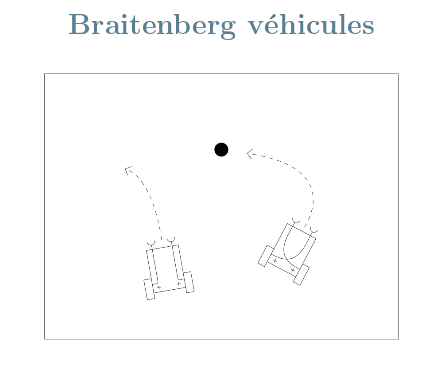
\includegraphics[width=10cm, height=10cm, keepaspectratio]{Braitenberg.png}
		\caption{Véhicule Braitenberg.}
		\label{fig:Braitenberg}
	\end{figure}
\paragraph{}	
On peut voir à travers les âges, que plusieurs civilisations (Grecques, Chine, Égypte) on modélisé leur technologies comme leurs esprits. Horloges, Systèmes hydrauliques, systèmes téléphonique, hologrammes, ordinateur analogues sont tous des métaphores de l'intelligence humaines.

\paragraph{}
Voici plusieurs événements en ordres chronologiques qui sont très important a l'IA avec une petite descriptions.
\begin{itemize}


\item \textbf{Hobbes, 1588-1679}
`Grand-Père` de l'IA. la pensée est un raisonnement symbolique. Ces idées ont été poussés par Descartes, Spinoza, Leibniz

\item \textbf{Babbage, 1792-1871}
Machine analytique, premier design d'ordinateur general-purpose

\item \textbf{Thèse Church-Turing}
Toute fonction arithmétique peut être fait sur une machine de Turing ou en calculus lambda ou formes équivalentes. n'a pas encore été prouvé mais a été testé par le temps..
\item \textbf{McCulloch et Pitts, 1943}
on prouver qu'un thresholding simple pouvait être interpréter comme une neuronne. Ce qui pourrait être une base pour une machine Turing-complete.
\item \textbf{Samuel, 1952}
Programme qui joue au checkers
\item \textbf{Minsky, 1952}
apparition du concept de réseaux de neuronnes
\item \textbf{Newell et Simon, 1956}
Programme qui trouve des preuves en logique propositionnelle.

\item \textbf{Rosenblatt, 1958}
Premier travaux significatif sur le perceptron
\item \textbf{Bobrow, 1967}
STUDENT, programme qui peut résoudre de l'algèbre de niveau secondaire en language naturel

\item \textbf{1970-1980}
Beaucoup d'effort dans les \textbf{Systèmes experts}, qui ont pour but d'avoir beaucoup de connaissances de pointes dans un domaine en particulier, pour qu'un ordinateur puisse faire des tâches de manière autonomes.
\item \textbf{Winograd, 1972}
SHRDLU, système qui peut faire une discussion et faire des actions intelligentes dans un monde simulé en utilisant que du language naturel.
\item \textbf{Warren et Pereira, 1982}
CHAT-80, peut répondre a des questions de nature géographiques en language naturel.
\item \textbf{Buchanan et Feigenbaum, 1965-1983}
DENDRAL, programme qui propose des structure atomique plausibles pour des nouveau composés organiques
\item \textbf{Buchanan et Shortliffe, 1984}
MYCIN, programme qui fait le diagnostique de maladie infectieuse du sang, prescrit le médicament requis et explique sont raisonnement
\item \textbf{1980 plus ou moins}
arrivé du prolog
\end{itemize}
\section{Agents Intelligents}
l'IA sert a utiliser un raisonnement pour faire un action. Une amalgamation d'une méthode de perception, d'un raisonnement et d'un mécanisme d'action est un \textbf{agent}. Un agent agit dans un \textbf{environnement}, les deux se trouvant dans un \textbf{monde}.
\begin{figure}[!ht]
\centering
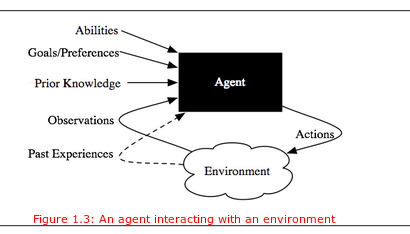
\includegraphics[width=5cm, height = 5cm, keepaspectratio]{Agent_base.png}
\caption{version generale d'un agent.}
\label{fig:Agentbase}
\end{figure}
\paragraph{}
Par exemple, un agent peut être un robot, son système de perception sont ces capteurs, sont processeur serait sa méthode de raisonnement et ses actuateurs serait sa méthode de mécanisme d'action. Son environnement serait son emplacement physique.Voici les différents types d'agents:

\begin{figure}[!ht]
\centering
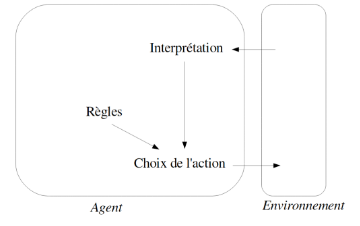
\includegraphics[width=5cm, height=5cm, keepaspectratio]{Agent_Reflexe.png}
\caption{Agent Réflexe}
\label{fig:agentreflexe}
\end{figure}
	

\begin{figure}[!ht]
\centering
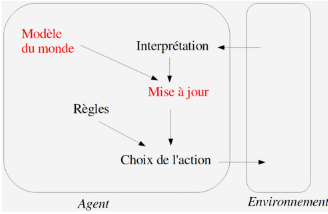
\includegraphics[width=5cm, height=5cm, keepaspectratio]{Agent_Memoire.png}
\caption{Agent Mémoire}
\label{fig:agentmem}
\end{figure}
	
\begin{figure}[!ht]
\centering
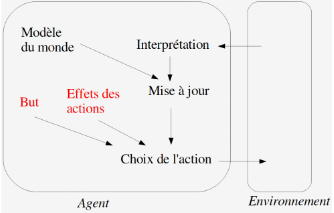
\includegraphics[width=5cm, height=5cm, keepaspectratio]{Agent_Memoire_But.png}
\caption{Agent Mémoire avec Buts}
\label{fig:agentmembut}
\end{figure}
	
\begin{figure}[!ht]
\centering
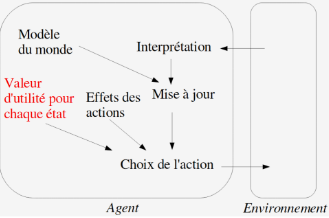
\includegraphics[width=5cm, height=5cm, keepaspectratio]{Agent_Memoire_Theorie.png}
\caption{Agent avec Théorie de la décision}
\label{fig:agenttheorie}
\end{figure}
\paragraph{}
Les agents qui peuvent apprendre sont d'une intérêt particulier. Ils peuvent eux-même changer leur comportement en fonction des échantillons d'entrainement grâces à des rétroactions positives et négatives.
\chapter{Méthode de Recherche dans un Espace d'États et Problème de Satisfaction de Contraintes.}
\section{Méthodes de Recherche dans un Espace États}
\paragraph{État}
ou dans le monde se retrouve l'agent dans sa recherche pour la solution. C'est en fonction de chaque problême. On utilise souvent une forme arborescent pour représenter sa position.
\begin{figure}[!ht]
\centering
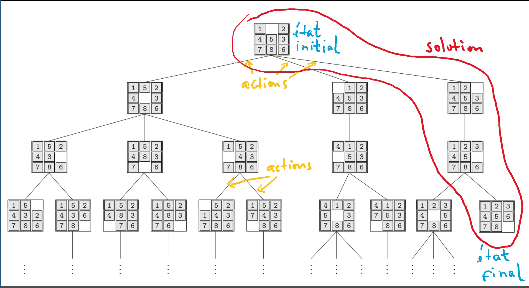
\includegraphics[width = 7cm, height = 7cm, keepaspectratio]{Etat.png}
\caption{Représentation d'un État}
\label{fig:etat}
\end{figure}

\paragraph{Fonction de Cout}
Normalement, on ne s'intéresse pas seulement a trouver une solution. On s'intéresse aussi a la qualité de la solution. On représente cela avec une fonction de cout. La convention est que le plus faible est la fonction de cout, le meilleur est la solution. Cette fonction associe une valeur a chaque action.

\paragraph{Méthode de recherche}
On définit une méthode de recherche comme étant le guideline qu'on utilise dans notre algorithme pour se déplacer dans notre espace d'états


\subsection{Méthodes de Recherche non informée}

\subsubsection{Méthode de Recherche en largeur}

La méthode de recherche en largeur cible a explorer toutes les noeuds possible de notre espace d'états sans prendre en considération la fonction de cout. Et en explorant toute les états de chaques étages de notre Arbre. Voir \ref{fig:Recherche_en_largeur} et \ref{fig:Algo_Recherche_en_largeur}

\begin{figure}[!ht]
\centering
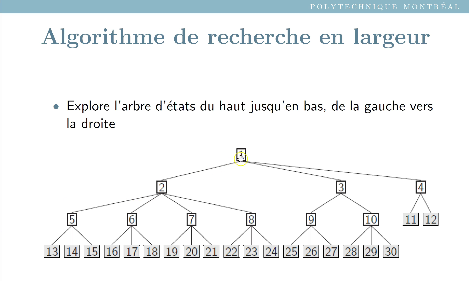
\includegraphics[width = 7cm, height = 7cm, keepaspectratio]{Recherche_Largeur.png}
\caption{Ordre d'exploration de la recherche en largeur.}
\label{fig:Recherche_en_largeur}
\end{figure}

\begin{figure}[!ht]
\centering
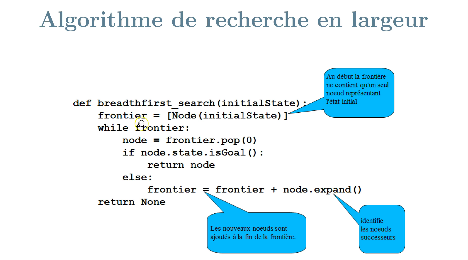
\includegraphics[width = 7cm, height = 7cm, keepaspectratio]{algo_largeur.png}
\caption{Algorithme de Recherche en Largeur.}
\label{fig:Algo_Recherche_en_largeur}
\end{figure}
\paragraph{Avantages}
on est sur d'avoir une solution. Et si tous les actions on le même cout, la solution sera optimale
\paragraph{Désavantages}
Le nombre d'état dans la frontière est très élevés.. Très grand temps de calculs et beaucoup de mémoire requis. On peut aider le problème de mémoire en prenant en considération les états déjà explorés

\subsubsection{Méthode de Recherche en profondeur}
\paragraph{}
La méthode de recherche en profondeur cible a expandre un noeud jusqu'à ce que l'état ne produit plus de nouvelle état ou qu'on trouve la solution. Si on arrive au fond. On change de branche et on commence a explorer un peu plus en largeur. Voir\ref{fig:Recherche_en_profondeur} et \ref{fig:Algo_Recherche_en_profondeur}

\begin{figure}[!ht]
\centering
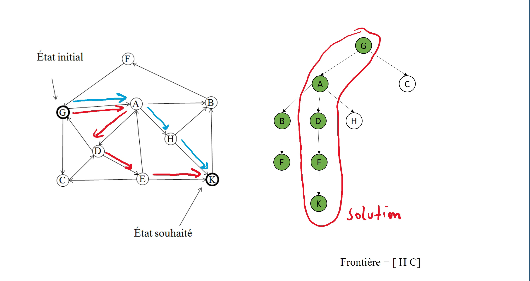
\includegraphics[width = 7cm, height = 7cm, keepaspectratio]{Recherche_Profondeur.png}
\caption{Recherche en Profondeur}
\label{fig:Recherche_en_profondeur}
\end{figure}

\begin{figure}[!ht]
\centering
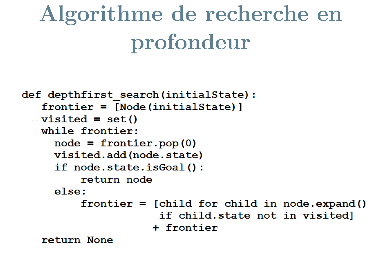
\includegraphics[width = 7cm, height = 7cm, keepaspectratio]{algo_profondeur.png}
\caption{Algorithme de Recherche en Profondeur}
\label{fig:Algo_Recherche_en_profondeur}
\end{figure}
\paragraph{Variantes Incrémentales}
On peut modifier l'algorithme de recherche en profondeur pour rectifier certains problèmes. Un des problèmes principales qu'on veut résoudre est que la recherche en profondeur peut se perdre dans une mauvaise ramification. On peut résoudre sa avec une approche incrémentale. C'est à dire, qu'on limite les solution qu'on explore en fonction de leur niveau.
\paragraph{}
Principale, on applique la recherche en profondeur avec des limites de profondeur de 1,2,3..n jusqu'à temps qu'on réussise a trouver notre solution. Sa évite que dans l'occurence qu'un problème à une très grande profondeur, qu'on se perd dans une super grande branche qui risque de ne pas donner de solution.
\paragraph{}
Cette solution n'est pas inefficace comme on l'imaginerait.. Cela est du au fait que la grande majorité du travail est fait lors du dernier niveau de l'arbre. Voir formule ci-dessous
\begin{align*}
N_{b}(D) &= \sum^D_{d=0} b^d = \frac{b^{D+1}-1}{b-1}
\end{align*}

\begin{itemize}
\centering
\item {b est le facteur de ramification}
\item {D est la profondeur de l'arbre}
\item {Nb est le nombre total de noeuds}

\end{itemize}

\subsubsection{Algorithme de Recherche a cout uniforme}

\paragraph{}
Les méthode de recherches en profondeur et en largeur ont tous les deux de grands désavantages qui rendent ces méthodes inutiles pour certains problèmes spécifiques. De plus, les deux algorithmes ne trouvent pas nécessairement la solution optimale.

\paragraph{}
L'algorithme de recherche à cout uniforme, malgré son nom un peu confusing, prend en compte de la fonction de cout. Fonction qui n'a pas nécessairement un cout uniforme.. \\

l'algorithme va toujours vouloir chercher les noeuds ayant une somme de couts minimales. Cette méthode va toujours donner une solution optimale. Par contre, elle risque d'explorer autant de noeuds que les méthodes de recherche en profondeur et en largeur. On peut considérer la recherche en largeur comme étant un cas particulier de la recherche a cout uniforme, si et seulement si la fonction de cout est égale pour chaque actions. Voir \ref{fig:Algo_Recherche_Uniforme} et \ref{fig:Recherche_Uniforme}

\begin{figure}[!ht]
\centering
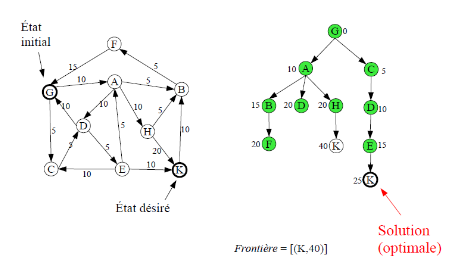
\includegraphics[width = 7cm, height = 7cm, keepaspectratio]{Recherche_Uniforme.png}
\caption{Recherche à cout Uniforme}
\label{fig:Recherche_Uniforme}
\end{figure}

\begin{figure}[!ht]
\centering
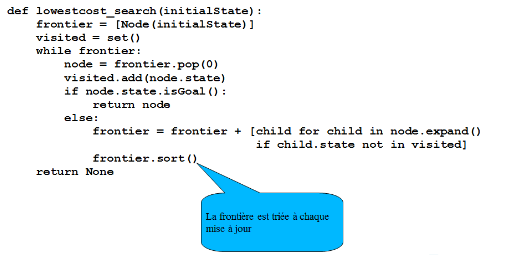
\includegraphics[width = 7cm, height = 7cm, keepaspectratio]{algo_uniforme.png}
\caption{Algorithme de Recherche a cout Uniforme}
\label{fig:Algo_Recherche_Uniforme}
\end{figure}

\subsubsection{Recherche Bidirectionel}
\paragraph{}
N'étant pas nécessairement un algorithme de recherche, la recherche bidirectionel est une facon de réduire le temps de recherche si on respect certain critères.
\begin{itemize}
\item Si on a une solution possible.
\item Si c'est possible de se rendre a la solution à partir de notre état d'origine, sinon notre solution et nos état initiale ne vont jamais converger.
\end{itemize}
 L'idée derrière la recherche bidirectionel est qu'on utilise notre algorithme de recherche dans les deux sens. Une fois en partant de l'origine pour se rendre jusqu'à la solution connus. La deuxième en partant de la solution pour essayer de se rendre jusqu'à l'état d'origine. \\
 
Normalement, on utilise une combinaison d'algorithme de recherche en profondeur partant de la solution et d'algorithme de recherche en largeur qui part de l'origine. Notre algorithme d'origine cherche a approfondire la frontière de noeud le plus largemene possible tandis que l'algorithme de notre solution cherche a la traversé. \\

Dans certains cas, nous allons avoir une amélioration. On peut la modélisé comme étant:
\begin{align*}
O_{initiale} &= b^{k} \\
O_{bidirectionel} &= 2b^{\frac{k}{2}}
\end{align*}
\begin{center}
ou b est le facteur de branchement et k la profondeur
\end{center}

\paragraph{}
Cependant, on assume toujours que nous sommes capables de rejoindre les frontières, ce qui n'est pas toujours le cas....

\subsection{Méthode de Recherche Informée}
\paragraph{Heuristique}
Une heuristique est une fonction qui essaie d'évaluer le potentiel d'un état donné en fonction de charactéristique distinctes à cet état. Ne pas confondre avec la fonction de cout, Celle-ci calcule le cout de l'état d'origine jusqu'à l'état actuel tandis que l'heuristique essaie d'estimer le cout de l'état actuel jusqu'à la solution.
\paragraph{}

par contre..
\begin{itemize}
\item Ce n'est pas garantie
\item Il faut que l'heuristique soit valide
\end{itemize}

On va s'en servir en l'incorporant dans notre algorithme de recherche, on va utiliser la fonction d'évaluation heuristique avec notre fonction de cout.\\

Pour trouver une bonne fonctions heuristiques, on peut soit parler avec un experts pour savoir quel sont les paramêtres les plus importants/qui peuvent être exploiter. \\

encore mieux, on peut aussi se servir de \textbf{l'apprentissage machine} pour pouvoir trouver nos paramêtre les plus statistiquement significatifs. Notre algorithme pourrait même ajuster son heuristique en fonction de sa.

\subsubsection{Heuristique Glutone}
\paragraph{}
Cet algorithme ne prend que l'heuristique en considération. On va s'en servir comme l'algorithme de recherche a cout uniforme sauf qu'au lieu de minimiser la fonction de cout, on va changer de voisins en prenant le voisins ayant l'heuristique la plus faible. Voir \ref{fig:Heuristique_Glutone} et \ref{fig:Prob_Heuristique_Glutone}

\begin{figure}[!ht]
\centering
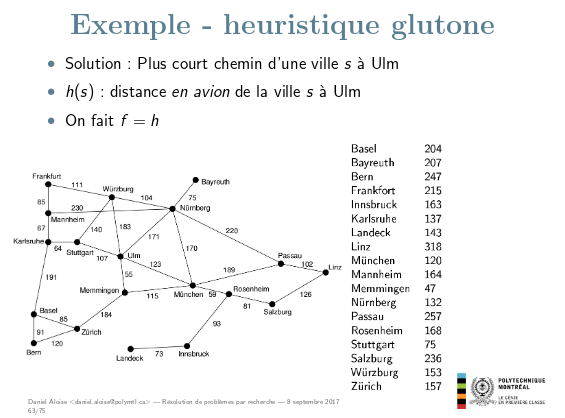
\includegraphics[width = 7cm, height = 7cm, keepaspectratio]{Heuristique_Glutone_Prob.png}
\caption{Problème d'heuristique glutone}
\label{fig:Prob_Heuristique_Glutone}
\end{figure}

\begin{figure}[!ht]
\centering
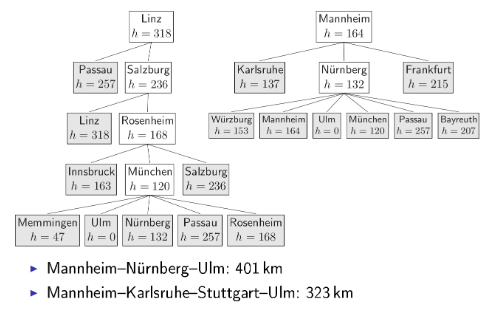
\includegraphics[width = 7cm, height = 7cm, keepaspectratio]{Heuristique_Glutone.png}
\caption{Prise de Décision de notre Heuristique Glutone}
\label{fig:Heuristique_Glutone}
\end{figure}

\subsubsection{Algorithme A*}
\paragraph{}
C'est algorithme ressemble grandement à l'algorithme de Recherche à cout uniforme. Cependant. Nous n'allons pas optimiser la fonction de cout, mais une fonction $f$ que nous allons définir comme étant
\begin{align*}
f(n) &= g(n) + h(n)
\end{align*}
\begin{center}
ou $g$ est notre fonction de cout défini dans la méthode de recherche a cout uniforme et $h$ comme étant notre heuristique. 
\end{center}


\paragraph{}
On peut alors déduire, qu'avec $h(n) = 0$ nous avons une recherche a cout uniforme et qu'avec $g(n) = 0$ nous avons une heuristique glutone. Voir fig.

\begin{figure}[!ht]
	\centering
	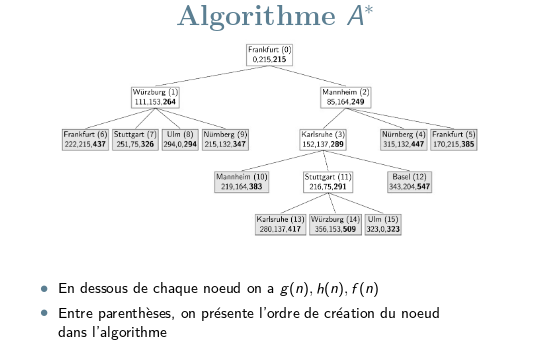
\includegraphics[width = 7cm, height = 7cm, keepaspectratio]{A*.png}
	\caption{Algorithme A*}
	\label{fig:A*}
\end{figure}
\paragraph{}
Par contre, pour que notre algorithme trouve une solution optimale, il faut que notre heuristique soit admissible. Soit:
\begin{align*}
g(x) = g(x) + h(x) \\
f(x) \leq f(z) \\
= f(x)\\
\leq f(z) \\
\leq g(z) + h(z) \leq g(y)
\end{align*}
pour fig\ref{fig:Preuve_A*}
\begin{figure}[!ht]
\centering
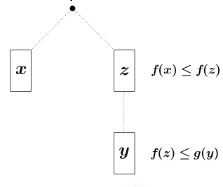
\includegraphics[width = 7cm, height = 7cm, keepaspectratio]{Preuve_A*.png}
\caption{Notre preuve pour A*}
\label{fig:Preuve_A*}
\end{figure}
\paragraph{}
Les faiblesse de l'algorithme A* sont 
\begin{itemize}
\item On peut avoir un grand nombre de noeuds à stocker
\item On doit les trier en plus à chaque itération (beaucoup de temps de calculs)
\end{itemize}
Pour régler ce problème, nous allons utiliser une recherche incrémentales.
\subsubsection{Variante A* incrémentale}
\paragraph{}
Cette variante est comme la recherche en profondeur incrémentale sauf qu'au lieu de limiter la profondeur, nous allons limiter la valeur de la fonction $f(n)$. Voir les figures 

\begin{figure}[!ht]
\centering
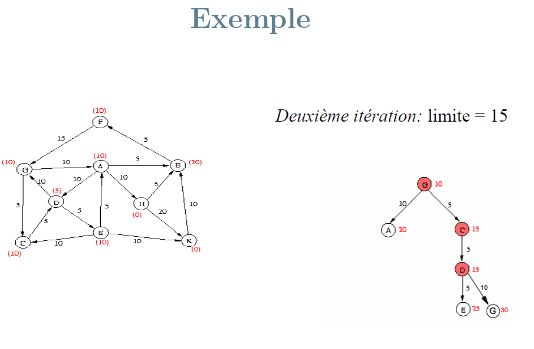
\includegraphics[width = 7cm, height = 7cm, keepaspectratio]{incrementale_15.png}
\caption{Limite de 15 dans l'approche incrémentale}
\label{fig:incrementale15}
\end{figure}

\begin{figure}[!ht]
\centering
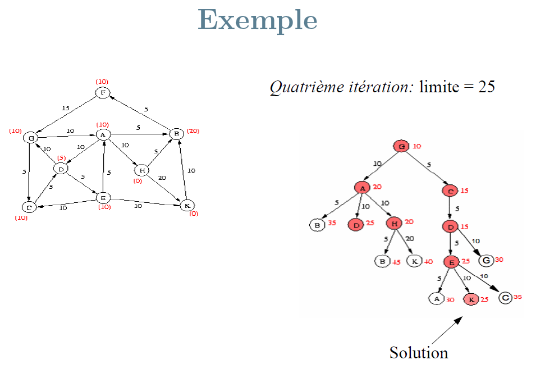
\includegraphics[width = 7cm, height = 7cm, keepaspectratio]{incrementale_25.png}
\caption{Limite de 25 dans l'approche incrémentale}
\label{fig:incrementale25}
\end{figure}
\subsection{Méthode de Recherche Locale}
\paragraph{Voisinage}
On appel un voisinage tous les noeuds qui peuvent être un successeur de l'état en question. pour revenir à notre analogie arborescente, le voisinage de l'état initiale serait l'étage en dessous. Le voisinage de tous les états du première étage serait les états du deuxième étage.. ainsi de suite.\\

Les méthodes de recherche locales ne conservent qu'un seul noeud en mémoire, celui ou nous sommes. En générale, avec une méthode de recherche locale on cherche seulement à trouver une solution, et non pas comment se rendre à la solution selon notre origine.\\

À chaque itération de notre algorithme, on remplace par notre meilleur noeuds jusqu'à temps qu'on a une solution. Normalement, on essaie de concevoir l'algorithme de sorte qu'il essaie de minimiser les conflits. Ou la solution possible est une solution sans conflit. \\

\noindent
Pour un voisinage étant défini comme un voisinage n-opt, cette fonction décrit l'ordre de complexité du voisinage.
\begin{align*}
O(n^k)
\end{align*}
\begin{center}
ou k est égale au nombre d'opérations permis
\end{center}

\paragraph{Randomisation} Si on peut trouver un bon optimum local avec un prob de $p$, une solution sera trouver en faisant $O(1/p)$ éxécutions.

\subsubsection{Recuit Stimulé} Le problème avec les méthodes généraliste de recherche locale est qu'il n'ont pas de notions de max-min local. C'est à dire, lorsqu'il va trouver un max ou un min, il ne sera pas si c'est le max-min globale, ou si c'est juste une max-min ordinaire(locale) 
\paragraph{Fait empirique:} Les bon optima locaux sont souvent près les uns des autres.\\

l'objectif de l'algorithme de recuit sitmulé est de laisser des solution mauvaise passer. Tout sa pour pouvoir sortir des différents max-min locale (voir fig \ref{fig:paysage_espace}

\begin{figure}[!ht]
\centering
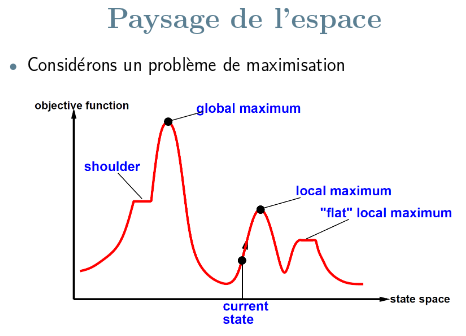
\includegraphics[width = 7cm, height = 7cm, keepaspectratio]{Paysage_Espace.png}
\caption{Exemple de Paysage de l'Espace. On cherche à trouver le maximum global sans rester pris dans un max locale}
\label{fig:paysage_espace}
\end{figure}
\paragraph{}
Au fur et à la mesure que le problème augmente en taille, le raport entre les mauvais et les bons optima locaux augmente (exponentiel). Ce qui rend le redémarrage de l'algorithme avec un départ différent futile. C'est la raison pourquoi on se sert du Recuit Stimulé. voir fig. pour algorithme.

\begin{figure}[!ht]
\centering
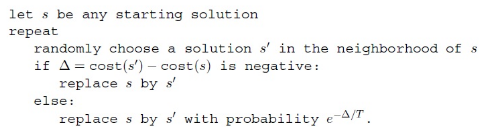
\includegraphics[width = 7cm, height = 7cm, keepaspectratio]{Recuit_Stimule.png}
\caption{Algorithme de Recuit Stimulé}
\label{fig:recuit_stimule}
\end{figure}
La difficulté avec le recuit stimulé est de trouver un bon régime de refroidissement pour T. Cet algorithme est rendu obsolete comparer a l'algorithme génétique.
\subsubsection{Algorithme Génétique}
\paragraph{}
L'algorithme génétique est très flexible. Dans le cours, il est considéré comme une recherche local tandis que certains expert le considère comme une recherche globale. \\

Le principe de l'algorithme génétique est de représenter ton problème/état comme étant une chaine de symbole (une entité). Nous avons besoin d'une quantité de solution possible, que nous allons appeller \textbf{population}. Nous essayer de répliquer la théorie de l'évolution sur cette population en appliquant des \textbf{croisements} et des \textbf{mutations}. Nous allons ensuite répéter le processus $n$ fois jusqu'à temp qu'un individu dans notre populations soit une solution qu'on désigne comme acceptable.\\

Voici les ligne directrice de l'algorithme génétique. (fig. \ref{fig:algo_genetique} et fig \ref{fig:exemple_algo_genetique} ) 

\begin{figure}[h!t]
\centering
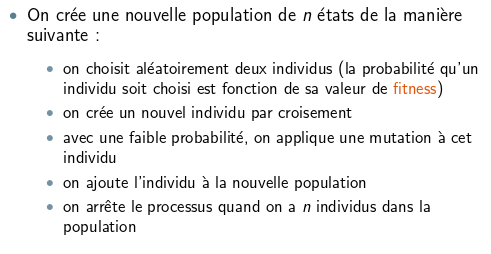
\includegraphics[width = 7cm, height = 7cm, keepaspectratio]{algo_genetique.png}
\caption{Ligne directrice de l'algo génétique}
\label{fig:algo_genetique}
\end{figure}


\begin{figure}[h!t]
\centering
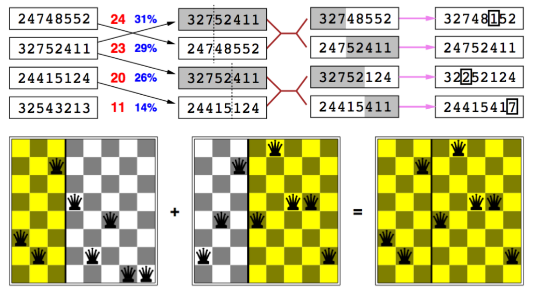
\includegraphics[width = 7cm, height = 7cm, keepaspectratio]{exemple_algo_genetique.png}
\caption{Exemple visuel d'algorithme génétique}
\label{fig:exemple_algo_genetique}
\end{figure}
\paragraph{}
L'algorithme génétique est très flexible. On peut nous même déterminer notre processus de sélection des solutions optimales après avoir fait notre croisements et mutations. On peut sélectionner pour vraiment avoir une bonne diversité génétique dans notre population ou on peut s'assurer de vraiment choisir les solutions optimales. Par contre, il faut réaliser qu'il est difficile de générer de meilleurs solutions si notre populations est hétérogènes. Alors il faut quand même s'assurer d'avoir des solutions qui ne sont pas nécessairement optimale, mais différent au point de vue du génotype.\\

voici sur la prochaine page quelques exemples d'opérateur de croisement et de mutations.
\begin{figure}[h!t]
\centering
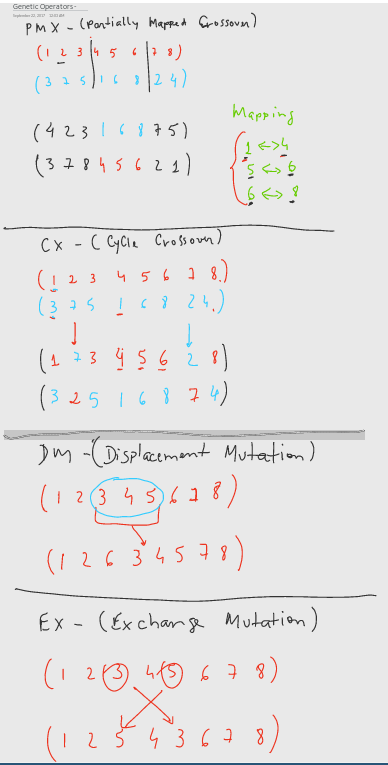
\includegraphics[height = 15cm, keepaspectratio]{operateur_genetique.png}
\caption{Exemple d'opérateurs génétiques}
\label{fig:ops_genetique}
\end{figure}
\section{Problème de Satisfaction de Contraintes}
\noindent Quoique très courte, cette section reste quand même très importante. \\
On formule un problème de satisfaction de contraintes comme suit:\\

\noindent un état est défini par $n$ variables $X_i, i = 1...n$ \\
\noindent Ces valeurs appartienne à un domaine $D_i$ \\

Cette formulation mène à la création d'algorithme généraliste. Le principe est de trouver une solution qui satisfait toute les contraintes appliquer sur les variable $X_{i\rightarrow n}$. Par contre, sa peut être utile d'analyser le problème à l'aide d'un graphe de contraintes.\\

\noindent On peut classer les contraintes par type. Ou: \\
\noindent \textbf{unaire} $\rightarrow$ s'applique à une seul variable\\
\noindent \textbf{binaire} $\rightarrow$ s'applique à deux variable\\
\noindent \textbf{ordre supérieur} $\rightarrow$ s'applique à plusieurs variables... très simple\\
\\subsection{Recherche Standard}
On défini la recherche standard comme:
\noindent \paragraph{état initiale:} l'affectation vide
\noindent \paragraph{successeurs :} affect une valeur à une variable pas affecté sans ajouter de conflits avec les affectations précédente $\rightarrow$ si ce n'est pas possible, la ramification est coupés. 
\noindent \paragraph{test de finitude :} l'affectation de variable complète.\\

c'est le même algorithme pour tous les problèmes, on suppose que le chemin pour se rendre à la solution n'est pas important. 

\begin{figure}[!ht]
\centering
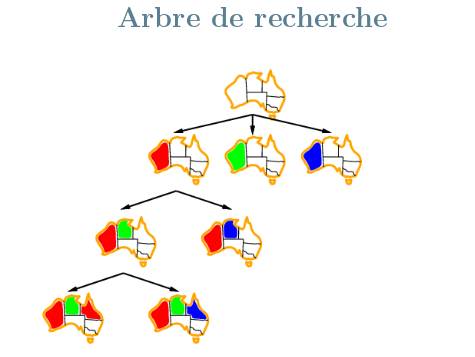
\includegraphics[width = 7cm, height = 7cm, keepaspectratio]{arbre_recherche_standard.png}
\caption{Arbre de Recherche Standard}
\label{fig:arbre_recherche_standard}
\end{figure}
\subsection{Backtracking}
Dans le cas ou notre algorithme prend une mauvaise branche par accident. On doit utiliser le backtracking pour revenir sur nos pas et pour pouvoir prendre la bonne branche.
Ce processus est inneficace. on finit par faire une recherche qui regarde une bonne partie des possibilités de notre arbre d'état. Ce qui en revient à faire une recherche en profondeur... \\
Pour pouvoir améliorer notre backtracking, on peut utiliser plusieurs méthodes.

\subsubsection{Heuristiques dans le Backtracking}
On trouve une fonction heuristique pour chaque contraintes. Sa pourrait être quelques chose qui choisit une valeur pour ta variable qui génère le moins de conflits. Sa pourrait être aussi qu'on choisit la variable qui à le plus grande nombre de contraintes et de choisit une valeur qui génère le plus de possibilité dans toutes les contraintes.

\subsubsection{Forward-checking}
C'est très self-explanatory. Le principe c'est de regarder le domaine de chaque variable instancié, et que pour chaque valeur qu'on attribuerait, on regarde si on viole une contrainte. \\

Si c'est le cas, on la retire du domaine. on s'arrète quand le domaine d'une variable est vide. Par contre, on ne peut pas détecter toute les violations (Pour pouvoir détecter toutes les violations, il faudrait faire du forward checking d'ordre du nombre de variable dans notre domaine, ce qui reviendrait à faire une recherche en largeur..) voir fig \ref{fig:forward_checking}

\begin{figure}[!ht]
\centering
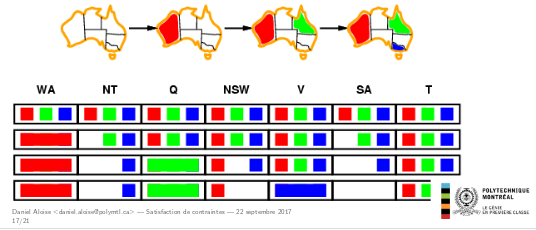
\includegraphics[width = 7cm, height = 7cm, keepaspectratio]{forward_checking.png}
\caption{Exemple de Forward Checking}
\label{fig:forward_checking}
\end{figure}

\subsubsection{Cohérence d'arc}
La dernière méthode de backtracking est la cohérence d'arc. Cette méthode en principe, regarde toute les variables et les compares avec toutes les autre variable. On compare toute les attributions de domaine, et on enleve toutes les valeur possible qui génère un conflit avec les autre valeurs de la variable à lequel tu la compare. On fait une comparaison avec toute les permutations de variables. voir fig \ref{fig:gac1}, \ref{fig:gac2}, \ref{fig:gac3} \\

\begin{figure}[!ht]
\centering
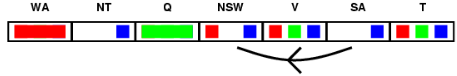
\includegraphics[width = 7cm, height = 7cm, keepaspectratio]{gac1.png}
\caption{Step1 GAC}
\label{fig:gac1}
\end{figure} 

\begin{figure}[!ht]
\centering
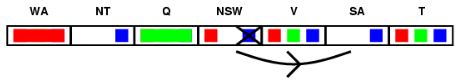
\includegraphics[width = 7cm, height = 7cm, keepaspectratio]{gac2.png}
\caption{Step2 GAC}
\label{fig:gac2}
\end{figure}

\begin{figure}[!ht]
\centering
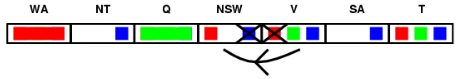
\includegraphics[width = 7cm, height = 7cm, keepaspectratio]{gac3.png}
\caption{Step3 GAC}
\label{fig:gac3}
\end{figure}
\chapter{Logique Propositionelle et Prédicat du Premier Ordre}
\section{Logique Propositionelle}
Apparament, en tant qu'humain on sait des choses. C'est chose pour être interpréter comme étant des connaissance sur le monde. On opère en fonction de ces connaissance et non en fonction d'un pure réflexe (voir Réseau de Neurones). On utilise un \textbf{raisonnement} basé sur nos \textbf{connaissances}. Jusqu'à dâte, nos méthode de recherches sont basé sur des problèmes très spécifiques.\\

Un Agent logique suit un framework comme suit:\\

\begin{figure}[h!t]
\centering
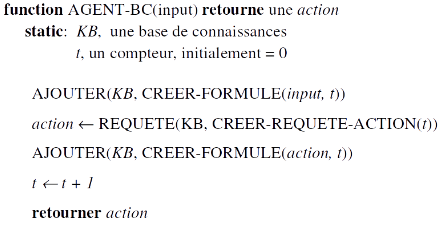
\includegraphics[width = 7cm, height = 7cm, keepaspectratio]{agent_logique.png}
\caption{Framework d'un agent Logique}
\label{fig:agent_logique}
\end{figure}

Le principe est que tu envoie la perception de ton agent dans sa base de connaissance. Ensuite en utilisant une méthode de référence, tu peux déduire certaines affirmations sur le monde. Ensuite, l'agent finit par redemander certaines affirmations sur le demande. Affirmations lequel la base de connaissance répond par un oui ou un non.\\

\noindent Un agent logique utilise:
\begin{itemize}
\item un \textbf{language formel} qui lui permet de représenter de façon compacte plusieurs situations différentes (logique propositionel et logique de premier ordre)

\item une \textbf{base de connaissances} pour stocker les faits connus spécifiques aux problèmes

\item des \textbf{algorithme d'inférence généraux} pour déduire des nouveaux faits.
\end{itemize}

\subsection{Conséquence Logique}
On définit une conséquences logique comme une chose conséquence d'un autre
\begin{align*}
KB \models \alpha
\end{align*}
\noindent est vraie si seulement si $\alpha$ est vrai dans tous les monde ou $KB$ est vrai aussi.

\noindent Exemple: $ KB = ( x = 3 ), KB \models ( x + 2 = 5 )$

On dit que $KB$ est un modèl de $\alpha$ dans la condition d'en haut.. On pourrait élaborer et dire qu'un modèle d'un affirmation $\alpha$ serait en fait une possibilité de représentation du monde.. voir fig 

\begin{figure}[h!t]
\centering
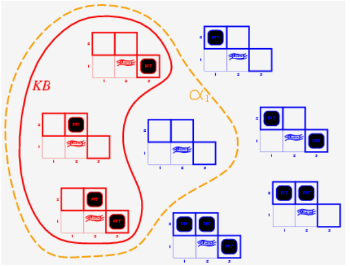
\includegraphics[width = 7cm, height = 7cm, keepaspectratio]{exemple_model.png}
\caption{Exemple d'un model}
\label{fig:exemple_model}
\end{figure}
\subsection{Syntaxe de la Logique}
la logique propositionnelle suit des règle très spécifique avec sa propre famille d'opérateur. En voici des exemples.\\

\begin{itemize}


\item Le connecteurs : $\wedge$,
$\vee$,
$\Rightarrow$,
$\Leftrightarrow$,
$\neg$ ont tous des fonctions specifiques 
\item pour S, nous avons $\neg$ S qui donne sont inverse (negation) implique $\neg$ S est vraie si S est faux
\item pour $S_1 et S_2$, on a $S_1 \wedge S_2$ si $S_1$ est vraie et $S_2$ est vraie
\item pour $S_1 et S_2$, on a $S_1 \vee S_2$ si $S_1$ est vraie ou $S_2$ est vraie
\item pour $S_1 et S_2$, on a $S_1 \Rightarrow S_2$ si $S_1$ est faux ou $S_1$ est vrai, \\
ie. c'est faux si $S_1$ est vraie et $S_2$ est faux
\item pour $S_1 et S_2$, on a $S_1 \Leftrightarrow S_2$ qui est equivalent a $S_1 \Rightarrow S_2$ et $S_2 \Rightarrow S_1$ 

\end{itemize}

Notre base de connaissance va être former d'une multitude de statements sous forme $X_1 \vee X_2 \wedge \neg X_3$ ou les variables X sont des variable qui représente certains aspects du monde. Comme par exemple sa pourrait représenter l'état d'une switch dans un circuit ou $True$ serait égale à un courant qui passe dans la switch et que $False$ serait lorsque rien ne passe dans la switch.\\


à l'aide de la syntaxe de la logique et de notre base de connaissance composés d'une multitude  de statements sur le monde. Il est possible de faire des déductions sur le monde basé que sur les statements dans notre base de connaissances.\\

On peut déduire une affirmation $\alpha$ de KB et l'écrire sous la forme : \\
\begin{center}
$ KB \vdash \alpha$
\end{center}

voici quelques règles d'inférence qui est valable:
\begin{align}
\neg(A\vee B) \vdash (\neg A\wedge \neg B) \textbf{      Loi de de Morgan}\\
\neg(A\wedge B) \vdash (\neg A \vee \neg B) \textbf{       Loi de de Morgan}\\
[(A \Rightarrow B), A] \vdash B \textbf{        Modus Ponens}\\
[(A \Rightarrow B), \neg B] \vdash \neg A \textbf{        Modus Tolens}\\
(A \wedge B) \vdash A \textbf{       Élimination du } \wedge\\
(A \Leftrightarrow B) \vdash (A\Rightarrow B) \wedge (B\Rightarrow A)\\
[(A \vee B), \neg A] \vdash B
\end{align}

\subsection{Inférence}
Pour faire de l'inférence, nous n'avons qu'à appliquer les formules vu ci-haut. On définit:
\paragraph{Algorithme de résolution :} Les formules sont normalisé et on applique une règles de résolution que nous allons voir plus bas

\paragraph{Formes Normale Conjonctive} Une formule est en FNC si et seulement si elle consiste d'une conjonction de clauses ou une clauses est une disjonction de littéraux. Un littéraux peut être vraie ou faux.
\begin{align}
FNC = K_1 \wedge K_2 \wedge K_m \\
\text{K est une clause} \rightarrow K_i = L_1 \vee L_2 \vee L_m\\
\text{ou L est un littéraux, vraie ou faux}\\
\text{forme finale = } (L_{11}\vee L_{12})\wedge (L_{21} \vee L_{22})
\end{align} 

\noindent Toute base de connaissance en Logique Propositionelle peut être traduite en Forme normale conjonction à l'aide de:\\ \\
\centering
$(A \Rightarrow B) \vdash \neg A \vee B$
\justify

\noindent On utilise ensuite la loi de De Morgan pour rendre les statements en une combinaise de $\vee$ et de $\wedge$. voir fig.\ref{fig:exemple_inference}

\begin{figure}[h!t]
\centering
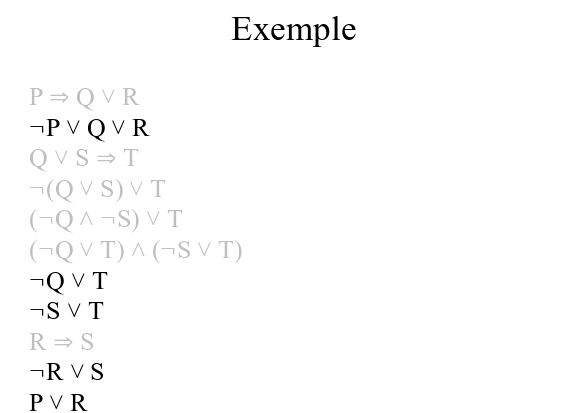
\includegraphics[width = 7cm, height = 7cm, keepaspectratio]{exemple_inference.png}
\caption{Exemple d'une traduction de statements en FNC}
\label{fig:exemple_inference}
\end{figure}

\noindent La base de connaissance KB doit toujours être consistante. c-à-d quelle ne se contredit pas elle dans ses statements. Exemple avoir un statement $S_1$ et de vouloir rajouter $\neg S_1$

\noindent Nos algorithme d'inférence peut être classifier de deux manières:

\begin{itemize}
\item \textbf{Algorithme Complet} Si un fait est une conséquence logique de la base de connaissance, notre algorithme doit être capable de déduire ce fait.\\
Si $KB \models \alpha$ alors $KB \vdash \alpha$

\item \textbf{Algorithme Correct} Si l'algorithme d'inférence déduit un fait. Celui-ci doit être nécessairement une conséquence logique de la base de connaissance, c-à-d, qu'il n'invente pas des fausseté. \\
Si $KB \vdash \alpha$ alors $KB \models \alpha$
\end{itemize}

\subsubsection{Clause de Horn}
On peut être encore plus spécifique dans notre définitions d'une clause. Les \textbf{clauses de horné} est une ensemble de clauses il y a au plus un littéral positif. voir fig \ref{fig:horn} 

\begin{figure}[h!t]
\centering
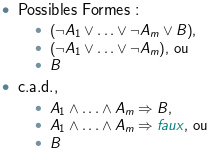
\includegraphics[width = 5cm, height = 5cm, keepaspectratio]{horn.png}
\caption{Formulation d'une clause de Horn}
\label{fig:horn}
\end{figure}

\noindent C'est important car en prolog, tout doit être défini par des clauses de horn.

\subsubsection{Chaînage Avant}
le premier algorithme d'inférence que nous allons voir est l'algorithme de chaînage avant. Le principe de l'algorithme est pouvoir déduire tout ce que nous pouvons avec notre base de connaissance, et ensuite de vérifier si nous pouvons déduire le statement que nous voulons, c-à-d $\alpha$. voir fig.\ref{fig:exemple_chainage avant} et \ref{fig:algo_chainage_avant}

\begin{figure}[h!t]
\centering
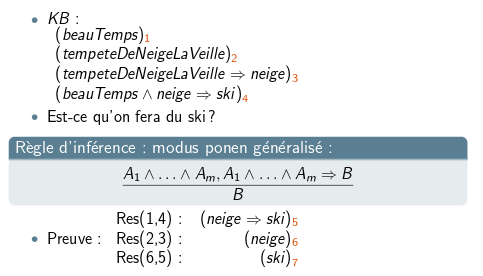
\includegraphics[width = 5cm, height = 5cm, keepaspectratio]{chainage_avant_exemple.png}
\caption{Exemple de chaînage avant}
\label{fig:exemple_chainage avant}
\end{figure}

\begin{figure}[h!t]
\centering
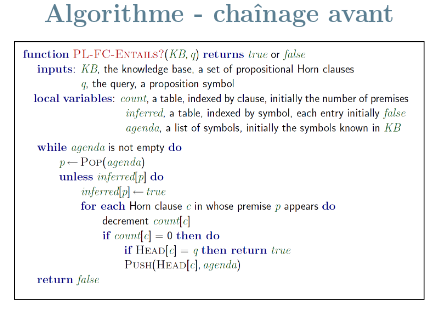
\includegraphics[width = 5cm, height = 5cm, keepaspectratio]{algo_chainage_avant.png}
\caption{Algorithme de chaînage avant}
\label{fig:algo_chainage_avant}
\end{figure}

\subsubsection{Chaînage Arrière}
Le deuxième algorithme d'inférence que nous allons voir est le chaînage arrière. cet algorithme essaie d'ajouter la négation du fait à prouver dans la base de connaissance. Si on fini avec une clause vide, sa veut dire que le fait qu'on essaie de prouver est faux (fig \ref{fig:exemple_chainage_arriere}). Il faut prendre garde. Car l'algorithme de chaînage passe les statements un à un de haut en bas. Il se peut que notre algorithme rentre dans une boucle infini si certains statements se font références (fig \ref{fig:chainage_arriere_loop}).\\

\begin{figure}[h!t]
\centering
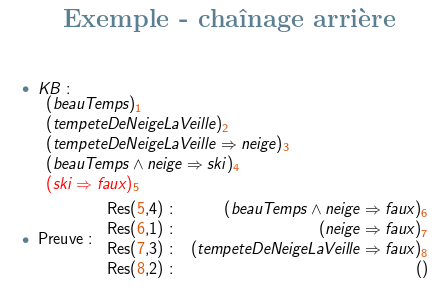
\includegraphics[width = 5cm, height = 5cm, keepaspectratio]{exemple_chainage_arriere.png}
\caption{Exemple d'un chaînage arrière}
\label{fig:exemple_chainage_arriere}
\end{figure}


\subsubsection{WalkSat}
Le troisième algorithme est le WalkSat. C'est en fait un algorithme très probabiliste. Sont principe est qu'on attribue aléatoirement des valeurs (vraie ou faux) à tous les littéraux présent dans notre base de connaissance qui pourrait faire matcher notre base de connaissance avec le statement à prouver $\alpha$. \\

Par contre, le désavantage avec sa, c'est qu'on peut 'tomber' dans un minimum local.. et qu'on ne peut jamais avoir une certitude que $\alpha$ est vraie.. En plus, le temps requis pour appliquer WalkSat peut être très grand étant donnée sa nature purement aléatoire. 

\section{Logique Prédicat du Premier Ordre}
La logique de Prédicat du Premier Ordre est très similaire à la Logique propositionelle. Par contre, il y a des différences notables. Le principe est qu'on fait une différence entre un objet et ses charactéristique et parfois même le contexte (une fonction genre père, mère..) .\\

\noindent On retrouve aussi la présence de quantificateur. Les quantificateurs sert à représenter les variables qu'on place dans nos prédicat. Voici quelques exemple:
\begin{align}
\forall X \rightarrow \text{veut dire}: \text{Pour tous les X, c'est absolue}\\
\exists X \rightarrow \text{veut dire}: \text{Il existe un X pour laquel la condition s'applique}\\
\end{align}
\noindent On retrouve aussi tous les opérateurs qu'on avait dans la logique propositionelle avec les mêmes signification, c'est à dire: $\neg , \wedge , \vee , \Rightarrow , \Leftrightarrow , =$
\noindent Voici quelques exemples de fonctions de prédicats avec leur significations

\paragraph{Tous les élèves sont intelligents} $\forall x [eleve(x) \Rightarrow intelligent(x)]$
\paragraph{Il existe un professeur intelligent} $\exists x [professeur(x) \Rightarrow intelligent(x)]$
\paragraph{Si un prof enseigne l'IA, il est intelligent} $\forall x [professeur(x) \wedge enseigne(x, IA) \Rightarrow intelligent(x)]$
\paragraph{Tout le monde aime tout le monde}$\forall x \forall y [aime(x,y)]$
\paragraph{Tout le monde aime quelqu'un}$\forall x \exists y [aime(x,y)]$
\paragraph{Quelqu'un aime tout le monde}$\forall x \exists y [aime(x,y)]$
\paragraph{Quelqu'un aime quelqu'un}$\exists x \exists [y aime(x,y)]$
\paragraph{Quelqu'un aime tous les prof d'IA}$\exists y \forall x [enseigne(x, IA)\wedge professeur(x) \Rightarrow aime(y, x)]$
\paragraph{Paul est un barbier qui rase tous cex qui ne se rasent pas}
$barbier(Paul) \\ \forall x[\neg rase(x,x) \Rightarrow rase(Paul, x)]$ 
\paragraph{Les brésiliens ne dansent pas tous la samba}
$\neg \forall x [bresilien(x) \Rightarrow danser(x, samba)]$\\
ou \\
$\exists x [bresilien(x) \wedge \neg danser(x, samba)]$

\subsection{Résolution}
Pour faire la résolution de problème en Logique de prédicat, on applique exactement les mêmes rêgles qu'avec la logique propositionnelle. On peut faire du chaînage avant en déduisant ce que l'on peut et on peut faire du chaînage arrière en plaçant l'inverse de notre statement dans notre base de connaissance. Évidemment, étant donné la quantification qui se rajoute, certaines modifications devront avoir lieu pour que tous puisse marcher normalement. C'est pour sa qu'on utilisera la \textbf{skolémisation} pour pouvoir résoudre ces problèmes. 

\subsection{Skolémisation}
 Le but de la skolémisation est d'éliminer les quantificateurs existentiel. En faisant sa, on change notre problème de sorte qu'on puisse les régler de la même manière que la logique propositionelle.\\
 
Voici un exemple de skolémisation pour résoudre un problème.\\

\noindent KB:\\
$\forall x [professeur(x) \Rightarrow \exists y \text{ } cours(y) \wedge enseigne(x, y)]$\\
$\forall x [cours(x) \Rightarrow \exists y \text{ } siteweb(y) \wedge associe(x,y)]$\\
$professeur(michel)$\\

\noindent On veut déduire $\exists y$ $siteweb(y)$
\noindent Voici les étapes requis pour faire la déduction
\setcounter{equation}{0}
\begin{align}
professeur(x) \Rightarrow cours(C_1(x))\wedge enseigne(x C_1(x))\\
cours(x)\Rightarrow siteweb(C_2(x))\wedge associe(x, C_2(x))\\
professeur(michel)\\
cours(C_1(michel))\\
enseigne(michel, C_1(michel))\\
\mathbf{siteweb(C_2(C_1(michel)))}\\
associe(C_1(michel), C_2(C_1(michel))
\end{align}

On peut voir qu'on vient de prouver ce qu'on voulait, c-à-d. qu'il y a un quelconque siteweb y qui existe

\chapter{Ontologies, Planification et Réseaux Bayésiens}
\section{Ontologies}
Quoique très philosophique, l'Ontologies est toutefois essentielle à la construction d'une base de connaissance cohérente. Le principe d'une Ontologies est en fait de classer nos prédicats en une hiérarchie de classe, pour qu'on puisse représenter non seulement comme un somme d'affirmations sur le monde, mais aussi comment relier ces affirmations pour qu'elle on un sen entres-elles.\\

On modélise des connaissance ontologiques avec un sens différentde la philosophie. On représente des classes en regroupant les entités sous forme de class.\\

une classe est une ensemble d'objet qui partagent certaines propriétés communes. On peut dire que certains objets partagent certaines caractéristique. Et comme mentionné sous haut, certaines classes ont des liens entres elle.\\

Les classes peuvent aussi former une taxonomie, comme par exemple, un animal est un être vivant (hiérarchie). Voici un exemple de taxonomie.fig \ref{fig:taxonomie}
\begin{figure}[!ht]
\centering
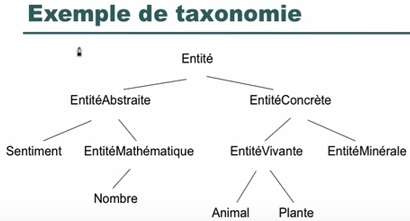
\includegraphics[width = 7cm, keepaspectratio]{taxonomie.png}
\caption{Exemple d'une taxonomie}
\label{fig:taxonomie}
\end{figure}

Maintenant, comment représente-t-on cela en logique? \\

On peut représenter les classes en utilisant des prédicats. Comme par exemple, je fait partie de la classe étudiant, Mr. Aloise, un professeur, etc. \\

Il faut que l'individu et sa classe soit lié. 
\paragraph{réification}
Une classe peut être sous-class d'une autre classe (voir fig \ref{fig:taxonomie}.)\\

On représente la hiérarchie en utilisant une clause. Comme par exemple. \\
animal(X) $\leftarrow$ mammifère(X)\\
animal(X) $\leftarrow$ oiseau(X)\\

Avec sa, on peut inférer que tweety qui est un oiseau, est un animal ! Par contre, si on utilise la forme réifier, sa ressemblerait a sa:\\

class(animal)\\
class(mammifère)\\
class(oiseau)\\
subclass(mammifère, animal)\\
subclass(oiseau, animal)\\

Sa montre que mammifère et oiseau sont des sous-classes de animal.. Par contre, il faudrait ajouter une règle pour dire qu'un animal ne soit pas un oiseau (car c'est impossible). \\

On a dit que les éléments d'un classes partagent certaines propriétés. On ne pourra jamais symboliser toute les subtilité, mais voici comment on fait pour représenter certaines caractéristique:\\

\begin{figure}[!ht]
\centering
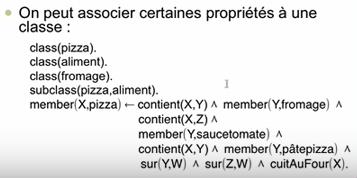
\includegraphics[width=7cm, keepaspectratio]{caracteristique.png}
\caption{représentation de certaines caractéristique d'une pizza}
\label{fig:caracteristique}
\end{figure}

Pour appeller plus loins, on peut représenter la disjonction entre certaines classes, comme par exemple, on ne peut pas être un animal et une plante. On peut aussi représenter les caractéristique des propriété elle-même.

\paragraph{réflexivité}
Le fait que un soit l'autre implique que l'autre soit un (commutativité). Si paul est au même endroit que Marie, Marie est au même endroit que Paul. \\

MemeGrandeur(X,X) $\leftarrow$ memeGrandeur(X,Y)

\paragraph{substances}
Le fait qu'une partie d'une classes peut on ne peut pas être un membre de cette classe elle-même.

\paragraph{transitivité}
Si X est plus grand que Y, et que Y est plus grand que Z, alors X est plus grand que Z.

\paragraph{symmétrique}
X est voisin de Y, alors Y est voisin de X\\

\subsection{Sémantique}
On peut représenter une interpretation comme étant un triplet:\\

$I = (D,\phi, n)$ ou \\
\begin{itemize}
\item D est le domaine ou ses éléments sont des individus (symboles de notre domaine)
\item $\phi$ est un mapping qui associe chaque constante à un élément de D. Comme par exemple, le mot 'téléphone' qui représente un engine physique correspondant a la définition d'un téléphone (voir fig. \ref{fig:semantics2})
\item n est un mapping qui assigne chaque symbole prédiceux de notre domaine à une [Vraie, Faux]
\end{itemize}
l'exemple avec cette définition décrit aussi une constance c qui denote notre individu $\phi(c)$ ici c est un symbol mais $\phi(c)$ peut être n'importe quoi dans notre domaine. Voici un exemple pour mieux expliquer.

On a un monde avec les objets de la figure \ref{fig:semantics}
\begin{figure}[!ht]
\centering

\includegraphics[width = 3cm, keepaspectratio]{semantics.png}
\caption{objets}
\label{fig:semantics}
\end{figure}

Ils sont dessinés parce qu'ils sont des choses dans notre monde réels et non des symbols. on a notre pair de sciseaux, notre téléphone et notre pencil.\\
Supposons que dans notre language, on a les constantes sciseaux, téléphone et crayons. Nous avons aussi les prédicats bruyant, left\_of/2. 

\begin{figure}[!ht]
\centering
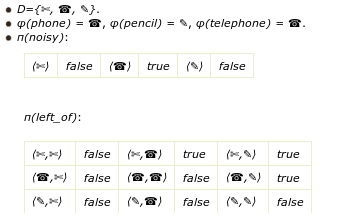
\includegraphics[width = 7cm, keepaspectratio]{semantics2.png}
\caption{Représentation d'un problème avec la sémantique}
\label{fig:semantics2}
\end{figure}

\subsection{interprétation}
Quand une variable apparait dans une clauses, la clause sera vraie pour n'importe qu'elle valeur qu'on peut associer à cette variable. Cette variable pourrait être décrite comme étant universellement quantifiable dans le scope de notre clause. si une variable X apparait dans notre clause C, on peut dire que C est vraie pour n'importe qu'elle association qu'on peut faire avec X (genre, les canadiens ? le souper de hier? n'importe quoi).\\

Pour définir formellement la sémantique d'une variable. On doit faire une assignation de variable $\rho$.. En ayant $\phi$ et $\rho$ on peut mapper chaque individu d'un domaine et pouvoir le manipuler avec la logique du prédicat..\\

voir :     http://artint.info/html/ArtInt\_281.html
\subsection{Partage des connaissances}
Avoir la base de connaissances et une représentation appropriés n'est seulement qu'un facette de notre agent. Il faut aussi que l'agent puisse en rajouter (voir apprendre) dans la base de connaissance. Soit par lui-même ou implanté directement dans la base de connaissance.\\

Cette aspects est vraiment importante quand la source d'information est très variés et à différents intervalles dans le temps. Le problème c'est que d'intégrer certaines bases de connaissances directement dans notre agent peut créer des conflits et une dissonnance. \\

Comme on l'a vue quelques paragraphes plus haut, une Ontologie est une manière de spécifier les moyens de représentations des symboles dans un système d'information. Un système d'information dans notre cas, sera notre base de connaissance ou n'importe quel autre source d'information (genre un thermometre??). On peut définir cette capacités de pouvoir intégrer et partager les connaissance d'une base de connaissance comme étant une \textbf{interopérabilités sémantique}. C-à-d, l'abilités de plusieurs différentes bases de connaissance de pouvoir travailler entre-elles.\\

Exemple, un agent d'achat peut confondre le mot 'chip' avec des croustilles (potato chips), des puces informatiques (computer chips), et retailles de bois (wood chips). La base de connaissance pourrait utiliser un moyen de représentation comme 'woodchip' ou 'woodchipmixed' pour représenter les retailles de bois.. Une compréhension du contexte est requis, sa prend un niveau d'abstraction assez élevé.\\

Voir :       http://artint.info/html/ArtInt\_312.html

\section{Planning}
On a vu dans le chapitre 1 certaines méthodes de recherches dans un espace d'états. Les méthodes reposait sur l'exploration d'un graphes et d'avoir un certains cout rattaché au mouvement effectué dans le graphe. Cependant, le graphe lui-même était bien défini. C-à-d., on sait à partir d'un noeud, quel sont les prochains noeuds qu'on puisse atteindre. Cela faisait en sorte que l'exploration d'un graphe était beaucoup plus axés sur la séquence d'actions à prendre à partir d'un état donné.
\subsection{Planificateur}
Maintenant, avec nos connaissance en logique de prédicat + Ontologies, on est capable de définir n'importe quoi de manière beaucoup plus précise.\\
Pour résumé, l'objectif de cette section est de faire un *merge* avec les méthodes de recherches dans un espaces d'état et la Logique de prédicat. Le but est de représenter nos états avec une base de données. Dépendemment des affirmations dans notre base de connaissance, certaines actions sont permissible et plusieurs autres états sont atteignable à partir de l'état présent.\\

\paragraph{PlanSAT} En terme de complexité, \textbf{PlanSAT} est la question de si une solution est possible dans un problème de planification. On peut aussi définir \textbf{BoundPlanSAT} comme étant le fait de trouver une solution dans un nombre $k$ d'itérations.\\

La réponse de PlanSAT est très orienter sur le nombre d'état possible. Les problèmes considérés \textbf{P-Space Hard} contiennent parfois une infinité d'états possible, alors théoriquement si aucune solution est possible, PlanSAT va rouler avec une durée infini en ne sachant jamais si une solution est possible ou non.\\



Exemple: On peut représenter un état initial comme étant:\\
At(TV, bestbuy)\\
At(truck, bestbuy)\\
At(driver, home)\\
path(home,amazon)\\
metro\_link(udM, CDN)\\

Le but de la planification, serait de déterminer tous les actions possible selon un état, et d'essayer d'en prendre une qui nous rapprocherait de notre but X, qui serait peut-être:\\

at(TV,home)\\

Pour faire cela, on serait peut-être obliger de faire quelques actions comme:\\

walk(driver,home,amazon)\\
load(TV,truck)\\
drive(truck, amazon, home)\\
unload(TV,home)\\
at(TV,home) - success\\


Un planificateur peut avoir à résoudre un problème d'un taille exponentiel. On s'en sert de la même manière qu'on fait une recherche dans un graphe. Par contre, les méthodes efficaces de recherches en graphes (A*) requiert la définition d'une heuristique. Et dans le cas d'un planificateur qui doit résoudre des problèmes de différentes natures, il peut être difficile d'établire une heuristique qui est efficace et qui reste admissible pour n'importe quel type de problème.\\

Chaque noeud de l'espace d'état est un état résultat de la prise d'une séquence d'actions  depuis l'état initiale. On peut appliquer une action A à partir d'un état S seulement s'il satisfait ses préconditions. Alors on peut définir l'application de A comme : \\

$S' = S - [\text{les effets de suppression de A}] + [\text{les effets d'addition de A}]$\\

\subsubsection{GPR}
La valeur de h(S) doit nous donner une estimation du nombre d'actions nécessaire pour transformer S en l'état final souhaité. Une heuristique très générale qu'on peut incorporer dans notre planificateur est celle du \textbf{Plans relâchés}, on plus communément, GPR.\\

L'idée est d'ignorer les effets de suppression, cela nous donne un aperçus de tout les états atteignable dans n prises d'actions. On construis un graphe composé de niveaux $S_0, A_0, S_1, A_1, S_2,A_2...$ qui représentent les états et actions possible. Le niveau $S_i$ détermine les actions qui peuvent être pris au niveau i tandis qu'au niveau $S_{i+1}$ contient les états atteignable à partir des états $S_i$. Quand on à tous les éléments requis pour notre but dans notre graphe à un certain niveau, on peut dire que notre but est atteignable dans ce même nombre d'actions.\\

Si on ne peut pas trouver l'état final souhaité à partir du \textbf{GPR} (plan relâché), on peut enlever ces états de notre recherches et explorer d'autre états. Par contre, c'est possible d'avoir un dead-end. c-à-d, d'avoir un état qui mène à la solution mais qui réalistement ne mène pas à la solution finale. Comme par exemple une série d'action qui donne un ensemble de connaissance C, mais que dans le processus normale, on enleverait une série d'action B faisant partie de C. Peut-être que la solution donné par notre GPR à besoin de B et C pour être trouver, ce qui n'est pas faisable.\\

On pourrait alors donné le nombre d'actions requise selon notre GPR pour atteindre un état but comme étant une heuristique valide. Cependant, c'est une heuristique qui est très cher à computer.. En pratique, on la combine avec la recherche locale pour augmenter son efficacité.

\subsection{PDDL}
Comme convention , on doit définir un problème:
\begin{itemize}
\item État Initiale
\item État Finale
\item Actions permissible, qui contient
\begin{itemize}
\item Action: Buy(x)
\item Precondition: At(Store), sells(Store,x)
\item Effect: Have(X), pays(??).. etc.
\end{itemize}
\end{itemize}

En théorie, un planificateur prend ces éléments, et avec un certains algorithme est capable de retourner un plan d'actions, plan qui permet a un individu à l'état initiale de se rendre à l'état finale.\\

Ce qui est très important, c'est que la programmation d'un planner est universelle, c'est la description du problème qui est unique à chaque instance. Cette modularité est très intéressante, car sa veut dire qu'un planificateur PDDL peut résoudre n'importe qu'elle problème qui est écrit en PDDL et un programme en PDDL peut être résous par n'importe quel planificateur qui à la capacité de résoudre un problème en PDDL.\\

On spécifie normalement un état comme une conjonction de termes, un état initiale dans un problème ne peut pas contenir aucune variable. Ces termes sont appelés fluent (parce qu'ils fluctuent?) et un état peut être vu comme un ensemble fluents qui doivent tous être vrais.


\paragraph{Hypothèse du monde fermé} Si un fluent n'apparaît pas dans un état, il est supposé faux.\\

On définit les actions en spécifiant leurs préconditions et leurs effets. Exemple:\\

\noindent
Fly(P,Orig, Dest)\\
PRECOND: At(P, Orig) $\wedge$ plane(P) $\wedge$ airport(Orig) $\wedge$ airport(Dest)\\
EFFECT: $\neg$ At(P, Orig) $\wedge$ At(P, Dest)

En spécifiant formellement les préconditions et les effets d'une action, on peut changer notre base de connaissance pour s'adapter au changement causer par notre actions. Comme par exemple le déplacement d'un objet, qui implique que la position d'un objet ne se trouve plus à la position initiale.\\

Voici un exemple de formalisation en PDDL d'un transport de marchandise.\\
\begin{figure}[!ht]
\centering
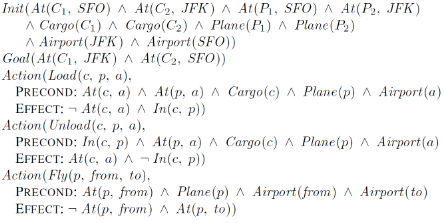
\includegraphics[width = \linewidth]{Exemple_Transport.png}
\caption{Exemple d'un transport de marchandise}
\label{fig:Exemple_Transport}
\end{figure}

en utilisant la formulation du problème et en utilisant un planificateur, on peut en extraire la solution suivante:\\

Load(C1,P1,SFO),Fly(P1,SFO,JFK),Unload(C1,P1,JFK)\\
\subsection{Exemple de Shakey le Robot}
\begin{figure}[!ht]
\centering
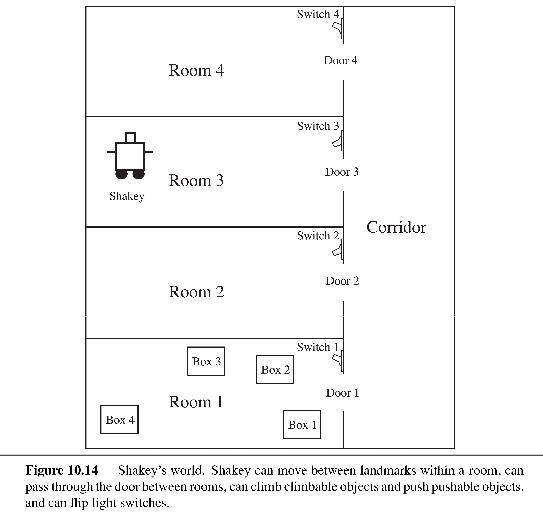
\includegraphics[width = 8cm]{Shakey.png}
\caption{Le monde de Shakey le robot}
\label{fig:shakey}
\end{figure}

l'objectif de l'exercices est de pouvoir modéliser les actions que Shakey peut faire dans sont mode, les voicis.\\

\begin{figure}[!ht]
\centering
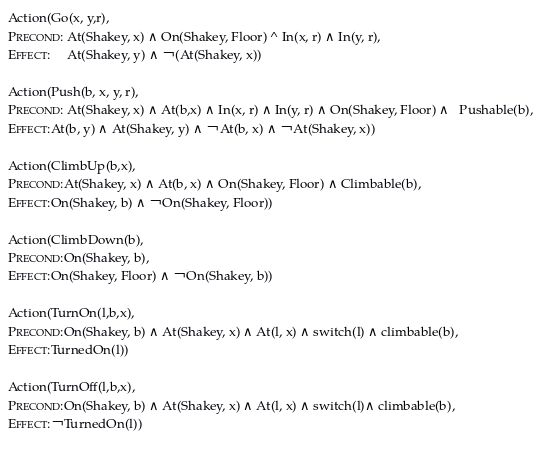
\includegraphics[width = \linewidth]{Reponse_Shakey.png}
\caption{Les actions que Shakey peut prendre}
\label{fig:Reponse_Shakey}
\end{figure}

\subsection{Sommaire}
Pour résumer, les planificateur sont des algorithmes très générale de résolution de problèmes qui fonctionnent sur des représentations explicites d'états et d'actions par des termes prédicatifs. On définit nos représentations et nos actions en PDDL, qui est un langage générale de définition de problèmes de planification. Ce planificateur opère comme un algorithme de recherche dans un espace d'états.

\newpage
\section{Réseaux de Bayes}
\subsection{Rappels des notions de bases}
Quelques définitions:\\
\begin{itemize}
\item On définit $\Omega$ comme l'ensemble de touts les résultats possible d'un événement. Comme par exemple un tir de dé: $\Omega = [1,2,3,4,5,6]$
\item chaque $\omega \in \Omega$ représente un résultat possible pour notre événement.
\item si les $\omega_i \in \Omega$ sont mutuellement exclusif et recouvrent $\Omega$, ils sont només événements atomiques.
\item Soit $\Omega = [\omega_1, \omega_2, \omega_3...\omega_n]$ fini, il n'y a pas de résultat préféré, ce qui signifie que nous supposons avoir la même fréquence d'occurence de chaque résultats, ce qui n'est pas souvent le cas en pratique. Dans le cas ou la probabilité est symmétrique, on peut définir la probabilité d'un événement comme étant :\\

\centering
$P(A) = \frac{|A|}{n}$\\
Pour avoir un nombre pair au dé:\\

$P(nombre \in [2,4,6]) = \frac{[2,4,6]}{[1,2,3,4,5,6]} = \frac{3}{6} = 0.5$
\justify
\end{itemize}

On peut aller beaucoup plus creux dans la réflexion. On peut avoir une \textbf{variable aléatoire} qui est une fonction des événements atomiques dans une ensemble de valeurs. \\

Notre fonction P induit une distribution pour une variable aléatoire X. on peut définir X comme étant une ensemble de valeur possible d'un événement et la fonction P(X) comme étant les chances qu'on obtienne la valeur dans la fonction. Comme par exemple:\\

\centering
$X = [A,B,C,D,E,F,G]$\\

on pourrait définir notre distribution de probabilité comme étant:\\

$[0.5,0.1,0.05,0.05,0.05,0.05,0.2]$\\

$P(A) = 0.5$\\

\justify
la somme de tous les probabilités dans notre distribution doit être égale à 1.\\

\paragraph{Distribution conjointe}
La distribution conjointe de probabilités fournit la probabilité de chaque combinaise possible des valeurs pour un ensemble de variable aléatoire.
\begin{figure}[!ht]
\centering
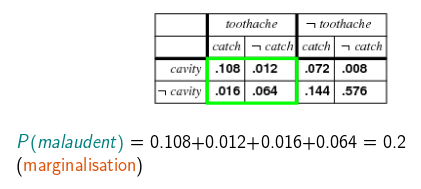
\includegraphics[width=7cm]{Distribution_Conjointe.png}
\caption{Exemple d'une distribution conjointe}
\label{fig:exemple d'une distribution conjointe}
\end{figure}

\paragraph{Probabilité Conditionelle}
La probabilité conditonnelle, noté P(a|b), signifie la probabilité de a étant donné que tout ce que nous savons sur le monde est b.

\begin{figure}[!ht]
\centering
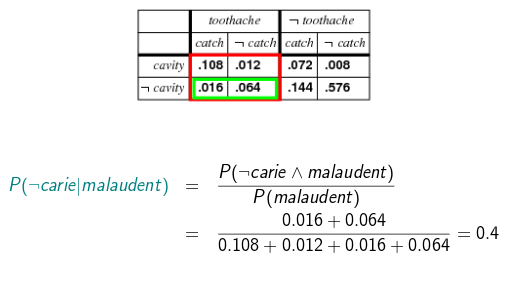
\includegraphics[width = 7cm]{Prob_Cond.png}
\caption{Exemple d'une probabilité conditionelle}
\label{fig:prob_cond}
\end{figure}

on peut définir plus formellement:
\begin{itemize}
\item $P(A|B) = \frac{P(A\wedge B}{P(B)} si P(B) \neq 0$
\item \textbf{Règle du produit} $P(A\wedge B) = P(A|B)*P(B) = P(B|A) * P(A)$
\item Règle de la chaîne : À faire
\end{itemize}

\paragraph{Indépendance des variables}
Deux variables sont indépendant si et seulement si:\\
\begin{itemize}
\item P(X,Y) = P(X)*P(Y)
\item P(X|Y) = P(X) et P(Y|X) = P(Y)
\end{itemize}

l'indépendant absolu est très puissant, mais en pratique c'est rare. l'odontologie en pratique est un domaine avec des centaines de variables qui ne sont aucunement indépendant, alors comment procédons-nous ?\\

\paragraph{Indépendance conditionelle}
Deux variables X et Y sont dites conditionellement indépendentes étant donné Z si:\\

\centering
P(X,Y|Z) = P(X|Z) * P(Y|Z)\\

ce qui est équivalent à aussi dire:\\

P(X|Y,Z) = P(X|Z)\\
P(Y|X,Z) = P(Y|Z)\\
\justify 

l'intuition est de dire que Si je sais que j'ai une carie, la probabilité que la sonde détecte ne dépend plus de si j'ai mal au dent. Donc:\\

\centering
P(detecte|malaudent, carie) = P(detecte|carie)\\
\justify

Bien que malaudent et Detecte soient tous les deux directement causées par Carie, aucune des deux a un effet sur l'autre. Par contre, sans cette connaissance a priori, les variables ne sont pas indépendantes.\\

Par équivalence:\\

P(malaudent|detecte,carie) = P(malaudent|carie)\\
P(detecte $\wedge$ malaudent | carie) - P(detecte|carie)*P(malaudent|carie)\\

\begin{figure}[!ht]
\centering
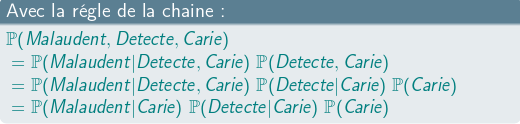
\includegraphics[width = 7cm]{Regle_Chaine.png}
\caption{Regle de la chaine}
\label{fig:regle_chaine}
\end{figure}

De facon générale, on utilise l'indépendance conditionelle pour réduire la taille de la représentation de la distribution conjointe de $O(e^n)$ à $O(n)$.

\paragraph{Théorème de Bayes}
En appliquant la règle du produit, soit :\\

\centering
P(A$\wedge$B) = P(A|B)*P(B) = P(B|A)*P(A)\\

\justify
on peut manipuler l'équation pour donner:\\

\centering
$P(A|B) = \frac{P(B|A) * P(A)}{P(B)}$

\justify
Cette relation est très utile pour évaluer la probabilité d'un diagnostique à partir de la probabilité causale. On peut généraliser cette équation pour nous donner quelques chose de plus intuitif, soit:\\

\centering
$P(Cause|Effet) = \frac{P(Effet|Cause) * P(Cause)}{P(Effet)}$\\

Comme exemple, soit:\\

$P(meningite|torticoli) = \frac{P(torticoli|meningite) * P(meningite)}{P(torticoli)} = \frac{0.8*0.0001}{0.1}$\\
\justify
\begin{figure}[!ht]
\centering
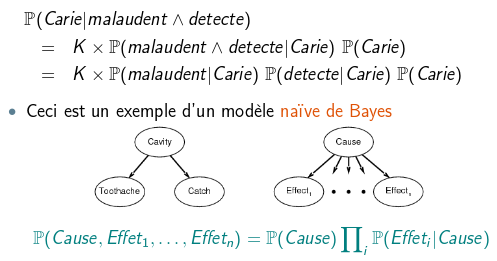
\includegraphics[width = 7cm]{Bayes.png}
\caption{Théorème de Bayes}
\label{fig:bayes}
\end{figure}
 
\subsection{Réseaux de Bayes}
Comme vue dans la section précédente, on peut définir une distribution conjointe comme représentant les probabilités d'occurence de plusieurs valeurs simultanés. Dans le cas ou les variables sont discrètes, le temps de calculs est proportionelle à $O(d^n)$ ou d est la quantité maximal de valeurs d'une de nos variables. Par contre, il faut connaître toutes les entrées et en pratiques, sa peut faire beaucoup de redondances en termes de calculs.\\

\subsubsection{Motivation}
Bob est célibataire et possède un système d'alarme installé dans sa maison pour se protéger de cambrioleurs. Bob ne peut pas écouter son alarme lorsqu'il est au bureau, donc il a demandé a ses voisin John et Mary de l'appeller si jamais l'alarme sonne. Après quelques années, Bob sait à quel point John et Mary sont fiable et il sait aussi que l'alarme peut être déclencher par un tremblement de terre. \\

En supposant que John et Mary ne peuvent pas regarder au dessus du mur pour voir si un cambrioleur est physiquement la:\\

\begin{figure}[!ht]
\centering
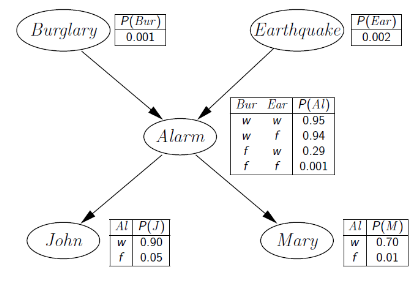
\includegraphics[width = 7cm]{bayes_network.png}
\caption{Notre Exemple}
\label{fig:bayes_network_exemple}
\end{figure}

De ce graphe, on peut faire plusieurs déduction. On peut premièrement voir que \textbf{Camrbiolage et Tremblement sont indépendant}. car peut importe quel variable on sait sur notre réseaux, la probabilité d'avoir un tremblebement de terre n'affectera pas la probabilité d'avoir un cambriolage ou vice-versa. Par contre, \textbf{si on sait que l'alarme à sonné, les probabilité de John et Mary sont conditionnellement indépendante} (car on sait l'alarme) vu que John et Mary n'auront aucun impact sur eux. Par contre, en ne sachant pas si l'alarme a sonner ou non, les deux événement ne sont pas indépendant car si John a appeller, c'est surement causer par un alarme ce qui influencera l'appel de Mary, ce qui falsifie l'indépendance.\\

l'intuition derrière les dépendences d'un graphe peut être facilement déduite. on peut traduire notre réseaux en un 'graphe d'indépendance' ou si deux variables sont reliés, elles sont indépendante. Lorsqu'un variable n'est pas connu, les liens entrant dans la variable connu est brisé tandis que les liens sortant y reste. ne sachant pas alarme, cambriolage et tremblement sont indépendant tandis que john et Mary ne le sont pas. Par contre, si on sait que l'alarme est déclenché, cambriolage et tremblement ne sont pas indépendant tandis que John et Mary son indépendant.\\

\begin{figure}[!ht]
\centering
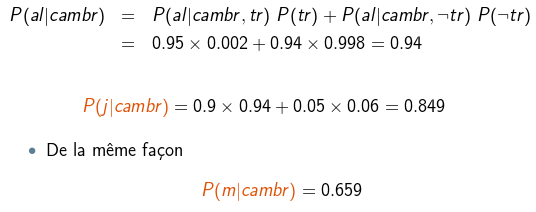
\includegraphics[width=7cm]{Exemple_Bayes.png}
\caption{Exemple Bayes}
\label{fig:Exemple_Bayes}
\end{figure}

\subsubsection{Explications}
Les réseaux de bayes nous permettent de résoudre des requètes en utilisant beaucoup moins d'espace mémoire et de temps de calculs. Le but des réseaux de bayes est d'explorer les connexions locales des variables.\\

dans un graphe, on peut dire que deux variable A et B sont indépendante ou conditionellement indépendantes si il n'existe aucune aretes entre elles, par contre, on ne peut pas dire que si il existe des arètes entre elles, qu'elle sont forcément dépendant, conditionelle ou non.\\

On peut formaliser les relations d'indépendances :\\

\paragraph{D-séparation}: critère générale pour décider si un noeud X est indépendant d'un noeud Y étant données d'autres noeuds $Z=[Z_1,Z_2,....Z_m]$. X est indépendant de Y sachant Z si tous les chemins non-dirigés entre X et Y sont bloqués par Z. On définit un chemin bloqué s'il contient au moins un noeud N qui satisfait une ou l'autre des conditions suivantes:

\begin{itemize}
\item il inclue un noeud $\rightarrow N \rightarrow$ ou $\leftarrow N \rightarrow$ ou $N \in Z$
\item il inclue un noeud $\rightarrow N \leftarrow$ et $N \notin Z$ et en plus qu'aucun des descendants de N peut appartenir à $Z$
\end{itemize}

Maintenant considérons un réseaux de Bayes sans cycles. En sachant les relations, on peut faire un tri topologiques de ses noeuds en sachant la directions des connections entre les différents éléments comme suit:\\

\begin{figure}[!ht]
\centering
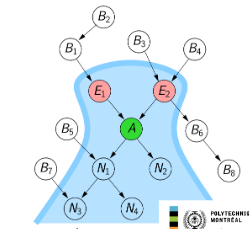
\includegraphics[width = 7cm]{tri_topologique.png}
\caption{tri topologique d'un réseaux de Bayes}
\label{fig:topologie_bayes}
\end{figure}

On peut alors représenter cette relations sous la forme d'une chaine de produit:\\

\centering
$P(X_1,....,X_n) = \prod\limits_{i=1}^n P(X_i|parents(X_i))$\\

\justify
Généralement, on fait sa en deux étapes après avoir choisit les variables qui sont nécessaire pour modéliser le domaine de l'application:\\

\begin{enumerate}
\item On choisit une ordre pour les variables.. soit $X_1,X_2,X_3,X_4...X_n$
\item on ajoute chaque variable dans notre graphes, en séléctionnant / ajoutant les parents et fils selon leur relation. Voir graphe ci-haut.
\end{enumerate}

l'ordre des variables joue un rôle très important. Une bonne stratégie est de partir des causes aux effets. Dans l'exemple qu'on a vu précédemment, il serait une mauvaise idée de partir avec les variables John et Mary étant donné que les autres variables ne sont pas impactés par leur performance.\\

Ultimement, c'est nous qui décide de l'ordre de nos variables ainsi que les relations parents/enfants, par contre, il faut ultimement fournir des probabilités pour chacune des relations, alors sa implique plus de travail, ce qu'on essaie ultimement d'éviter.

\subsection{Sommaire}
On définit un réseau de Bayes par:

\begin{itemize}
\item Un ensemble de variables et d'arètes dirigées entre ces variables
\item Ces noeuds et ces arètes forment un grpahe dirigé sans cycles
\item Chaque variable peut assumer un nombre fini de valeurs
\item Pour chaque Variable A, un tableau de probabilités conditionelles P(A|parents(A)) est donnée
\item Lors de la construction d'un réseau de Bayes, les variables doivent être classés selon le critère de la causalité.
\end{itemize}
\chapter{Machine Learning / Apprentissage Machine et Fouilles de données}
*nouvelle étagère*..\\

l'apprentissage machine peut être définir comme:
\begin{itemize}
\item une machine qui peut s'adapter ?
\item une capacité à se reconfigurer ?
\item qui évolue ?
\end{itemize}

en fait, pour être plus générale, l'apprentissage machine c'est la traduction du monde en un model. On traduit un ensemble de données dans une représentation différentes, qui ensuite peu être utiliser/ transformé pour être analyser. On retrouve cela sous plusieurs différentes formes, comme par exemple la reconnaissance d'image, l'analyse syntactique et autres. Sa dépend de quoi on parle. On peut représenter l'apprentissage comme une accumulation de règles sur quelques connaissances. Normalement, l'apprentissage machine exige un certain niveau de généralisation. \\

\paragraph{Apprentissage Supervisé}
Un type d'apprentissage ou on doit fournir certains exemples et que la machine essaie d'apprendre en analysant les exemples.\\

Exemple: Un producteur de fruit veut automatiquement divise ses pommes en catégories A et B. Le dispositif de tri est équipé de capteurs pour mesurer les \textbf{features} : la taille et la couleurs.\\

Avec ses features, la machine essaie de synthétiser une fonction pour qu'il puisse déterminer la catégorie dont laquel l'objet fait partie, soit A ou B, en utilisant seulement ses features. Normalement, on essaie d'avoir des features qui sont très simples.\\

\begin{figure}[!ht]
\centering
\includegraphics[width= \linewidth]{Classes_ML.png}
\caption{Exemple de catégorie}
\label{fig:Classes_in_ML}
\end{figure}

\begin{figure}[!ht]
\centering
\includegraphics[width = \linewidth]{Classes_division.png}
\caption{Exemple de division pour une classes}
\label{fig:Classes_division}
\end{figure}

Avec cette fonction synthétique, on est capable de prédire la catégorie de la pomme sans avoir besoin de l'utilisateurs. Par contre, on a besoin d'un échantillon initiale pour qu'il puisse déterminer la fonction lui-même. En pratique, on a beaucoup plus que deux features, alors les fonctions peuvent être très complexe. Cette fonction doit avoir une bonne performance pour classifier des nouveaux objets.\\

\begin{figure}[!ht]
\centering
\includegraphics[width= \linewidth]{Classifier_Agent.png}
\caption{Voici la forme de notre agent}
\label{fig:Classifier_Agent}
\end{figure}

*L’apprentissage machine est l’étude des algorithmes informatiques
qui s’améliorent automatiquement grâce à l’expérience - Mitchell 1997*\\

\textbf{Terminologie}
\begin{itemize}
\item Tâche : La tâche d’un algorithme d’apprentissage est de
apprendre une fonction menant d’un vecteur de
features à une valeur de classe, ex: couleur et taille $\rightarrow$ classe de la marchandise
\item Ensemble d'entraînement : contient les connaissances que
l’algorithme d’apprentissage est supposé d’extraire\\
*\\
d’habitude fournit par des experts
\item Ensemble de test : important pour évaluer si l’agent entraîné
peut bien généraliser ce qu’il a appris à de nouvelles
données
\item Mesure de Performance : ex. quantité de données bien classées, plus facile que de connaître la fonction apprise
par l’agent
\end{itemize}

C'est généralement plus facile d'évaluer la fonction synthétique que de la construire. \\

\paragraph{Apprentissage par renforcement}
l'agent améliore sa performance en fonction de ses interactions avec l'environnement. C'est un peu comme interpréter un feedback de l'environnement. Chaque action fait dans un environnement est associé a une récompense. On essaie d'avoir le plus de récompense possible. Le TP3 est un exemple d'apprentissage par renforcement (le fait que les fourmis aime la phéromone), la phéromone qui est donc le mécanisme de renforcement et influence le comportement des fourmis.\\

\paragraph{Apprentissage non-supervisé}
Apprentissage ou on a aucun information a priori. Soit de l'environnement ou fournie par un expert. On essaie quand même d'extraire des connaissances quand même.\\

Exemple, SVD, LSA, la réduction de dimension nous permet de déduire de la nouvelle information sans avoir besoin d'apprendre. voir LOG6308\\

\paragraph{Fouilles de données}
Le principe de fouilles de donées est un *parapluie* en dessous de l'apprentissage machine. C'est une manière de rendre les connaissance compréhensible pour les humains. C'est comme pouvoir interpréter les résultats ou les connaissance de nos machines, c'est une manière de comprendre les résultats.
\paragraph{Perceptron}
Rosenblatt- 1957, Il se base sur la neurones animales pour faire une machine\\
\begin{figure}[!ht]
\centering
\includegraphics[width= \linewidth]{Neurone.png}
\caption{Forme d'une neurone}
\label{fig:Neurone}
\end{figure}

Le principe est que si un signal d'entrée dépasse un certain niveau, la neurones transmet un signal à un autre neurones. *Beaucoup plus complexe, mais sa va venir*\\

Le perceptron, à la base, est un classificateur linéaire, qui suit la fonction:\\

$\sum_{i}^{n} a_i x_i =\theta$\\

ou on inscrit un hyperplan de n-1 dimension (fig. \ref{fig:exemple_hyperplan}):

\begin{figure}[!ht]
\centering
\includegraphics[width = \linewidth]{Hyperplan.png}
\caption{Projection d'un hyperplan pour notre classificateur}
\label{fig:exemple_hyperplan}
\end{figure}


On peut définir, un ensemble linéairement séparable comme un fonction ou on peut trouver un hyperplan pour lesquels les éléments d'une classe vont avoir une valeure plus petites que $\theta$ pour tous les x qui appartient a un ensemble et plus grand que $\theta$ pour un autre ensemble\\

$\sum\limits_{i=1}^{n} a_i x_i < \theta$\\

Pour tout x appartenant à $M_1$ et\\

$\sum\limits_{i=1}^{n} a_i x_i \geq \theta$\\

Pour tout x appartenant à $M_2$

Exemple: l'exemple à gauche est linéaire séparable tandis que celle de droite ne l'est pas. (fig. \ref{fig:lineairement_separable})\\

\begin{figure}[!ht]
\centering
\includegraphics[width= \linewidth]{lineairement_separable.png}
\caption{ }
\label{fig:lineairement_separable}
\end{figure}

Les neurones était abandonée jusqu'au années 90 parce qu'elle n'était pas capable de classifier la fonctions XOR. Elle tombe dans l'oublie.... \\

On réussi à combiner les neuronnes pour faire des réseaux de neurones afin de produire un classificateur non-linéaire. Tout récemment, il y a eu une grosse explosion qui a amener une popularité au réseaux de neuronnes, qui s'appelle \textbf{Deep Learning}. Ils sont devenu populaire en raison:
\begin{itemize}
\item leur facilité a paralléliser
\item les groupes d'investissement on rendu les chose très disponible, voir. Open Source. et c'est très facile a déployer
\item Ils ont remarqués que le Deep Learning était capable d'automatiser l'extraction des features. (automatiquement trouver la moyenne, la couleur.. ). et même aussi de déterminer quel features sont importants. Tout ce fait tout seul. 
\end{itemize}

\section{Maths}
On considère un entré x avec n charactéristique. avec x comme une combinaison linéaire de ses caractéristique.\\

$x = (x_1... x_n)^T$\\

$z = (w_i x_i...w_n x_n)$\\

ainsi que la fonction d'activation:\\

\centering
$
\phi (z)=
\begin{cases}
1 $ if $ z \geq \theta\\
-1 $ if not $
\end{cases}
$\\

Pour une question de simplicité, on peut faire:\\

$w_0 = - \theta$\\
$x_0 = 1$\\

ce qui donne\\

$z = w_0 x_0 + w_1 x_1 + ...w_n x_n $ et\\
$\phi (z) =
\begin{cases}
1 $ if $ z \geq 0\\
-1 $ if not $
\end{cases}
$
\begin{figure}[!ht]
\centering
\includegraphics[width = \linewidth]{Exemple_Perceptron.png}
\caption{Exemple d'un perceptron}
\label{fig:Exemple_Perceptron}
\end{figure}

\justify
L'algorithme de perceptron de base:\\

\begin{enumerate}
\item On initalise le vecteur de poid w avec des très petites valeurs.
\item Jusqu'à ce qu'on rencontre la condition désiré, on prend la valeur de notre sortie, on met a jours les poids, et on recommence jusqu'à temps que notre fonction ait le fonctionnement désiré
\end{enumerate}
Le processus de updater les poids est au coeurs de l'apprentissage profond.\\

$w \leftarrow w + \delta w^{(t)}$

La règle de l'apprentissafe du perceptron est donnée par :\\

\centering
$\delta w^{(t)} = \eta (y^{(t)} - \phi (z^{(t)})) x^{(t)}$
\justify

ou $\eta$ (entre 0 et 1) est le taux d'apprentissage et y est la classe connu de l'exemplaire x.\\

Le principe est qu'on met un objet dans notre fonction, on regarde la sortie et on la compare avec la catégorie attendu, si c'est bien, on passe à la prochaine item. Si c'est mal, on change les poids.. on fait sa pour tous les objets de notre ensemble d'entraînement.\\

\centering
$\delta w^{(t)} = \eta (1 -- 1) x^{(t)} = 2 \eta x^t$\\
et\\
$\delta w^{(t)} = \eta (-1 -1) x^{(t)} = -2 \eta x^t$\\
\justify
Exemple: si l'ensemble n'est pas linéaire séparable et qu'on essaie de la modéliser avec une fonction linéaire (en haut), on n'aura jamais la convergence. Si on essaie, on aura surement une sorte d'overfitting qui va augmenter la valeur des poids sans avoir d'augmentation de performances. \\

On ne peut guarantire la convergence que lorsque:\\
\begin{itemize}
\item les deux classes sont linéairement séparables
\item le $\eta$ est suffisament petit
\end{itemize}
On peut utiliser une sorte de seuil d'exécution si jamais les données d'entrainement ne sont pas linéairement séparables.\\

l'idée c'est d'utiliser la différence entre la valeur attendu et la valeur obtenue avec le taux d'apprentissage pour changer le poid de nos features dans nos modèles linéaires.

\subsection{Sommaire}
\begin{figure}[!ht]
\centering
\includegraphics[width = 5cm]{sommaire.png}
\caption{sommaire d'un perceptron, sous forme visuelle}
\label{fig:sommaire_ML}
\end{figure}
\section{Perceptron Adaptif}
Les poids sont mis à jours basés sur une fonction d'activation linéaire $\rightarrow$ différentiable
$\phi (w^T x) = w^T x$

Le principe est d'utiliser un quantificateur très similaire à la fonction d'activation du perceptron classique afin de prédire les classes.

\begin{figure}[!ht]
\centering
\includegraphics[width = \linewidth]{adaline.png}
\caption{model d'adaline}
\label{fig:adaline}
\end{figure}

\paragraph{Descente de Gradient}

On utilise la fontion ci-desous pour modéliser le processus d'apprentissage. Normalement, on essaie de minimiser : \\

$J(w) = 1/2 \Sigma _{t} (y^{(t)} - \phi (x^{(t)})^2$

Généralement, on essaie de converger dans un minimum local avec le gradient (le gradient représentant la direction vers lequel notre solution se dirige). Le problème est convexe alors il n'y a qu'un seul optimum local, qui est aussi l'optimum global.\\

\begin{figure}[!ht]
\centering
\includegraphics[width = \linewidth]{SGD.png}
\caption{visualisation d'une descente de gradient stochastique}
\label{fig:SGD}
\end{figure}
 on exprime d'abord:\\
 
\centering
$w \leftarrow w + \delta w$\\

\justify
ou plus précisément: \\

\centering
$\delta w = - \eta \nabla J(w)$\\

\justify
*on ajoute le 1/2 parce que dans le processus d'apprentissage, il y a un coefficient* A REVOIR\\

trouve le gradient en utilisant la dérivé partielle de J par rapport aux poids de chaques features, ce qui nous donnes: \\

\centering
$\frac{\partial J}{\partial w_i} = - \sum\limits_t (y^t - \phi (z^t)) x_i^t$\\
\justify
t = objets\\

Dans Adaline, on met à jour tous les poids d'une seule fois, pas par exemplaire d'entraînement.

\section{Regréssion Logistique}
Pour la régression logistique, on utilise la fonction logistique comme fonction d'activation. Au lieu d'avoir une fonction échelon, on utilise une fonction plus lisse..\\

C'est différentiable, convexe et beaucoup moins sensible aux outlier\\

$\phi (z) = \frac{1}{1+e^{-z}}$\\

\begin{figure}
\centering
\includegraphics[width = 5cm]{sigmoide.png}
\caption{fonction sigmoide}
\label{fig:sigmoide}
\end{figure}

Normalement, on utilise la fonction logistique pour modéliser une fonction de densité de probabilité tandis que la fonction échelon sert vraiment à classifier les objets.\\

On peut interpréter le résultats de la fonction logistique pour qu'il représente la probabilité qu'un objet appartienne a une classe. x comme étant notre facteur de confiance.\\

\begin{figure}[!ht]
\centering
\includegraphics[width= 8cm]{logistique.png}
\caption{ou y = quantizer}
\end{figure}

Normalement, pour la régression logistique, on essaie de minimiser \textbf{l'entropie croisée}, soit: \\

\centering
$J(w) = \sum\limits_t -y^t log(\phi(z^t)) - (1 - y^t)log(1-\phi(z^t))$\\
\justify

On essaie, comme le perceptron, de calculer le gradient de cette fonction afin de se rendre au minimum local. On peut même voir qu'en appliquant le gradient, on trouve a peu près la même règle d'apprentissage, soit:\\

$\delta w_i = \eta \sum\limits_t (y^t - \phi(z^t)) x_i^t$\\


Ou la fonction $\phi$ est la fonction logistique, au lieu de la fonction échelon..\\

\section{Descente de Gradient Stochastique}
La descente de gradient stochastique à le même principe que la descente normale, sauf qu'au lieu de calculer le gradient sur toutes les poids avec tous l'ensemble. On utilise une approche beaucoup plus incrémentales, c-à-d, on calcule le gradient pour un poid, avec un objet. sa veut dire qu'on entraine nos poids beaucoup plus rapidement, mais avec une direction beaucoup moins certaines. On n'essaie pas de converger directement vers un minimum, on prend un chemins \textbf{Stochastique} pour arriver à un minimum que l'on espère, globale.\\

on peut modéliser avec la formule :\\

\centering
$\delta w_i = - \eta \frac{\partial}{\partial w_i}J(w, t^*) = \eta (y^{t^*} - \phi(z^{t^*})x_i^{t^*}$\\

\justify
Cette procédure est beaucoup plus efficaces lorsque l'ensemble d'entrainement est grand. Par contre, le processus d'optimisation est moins efficace, ce qui est voulu. \\

\paragraph{solution intermédiaire} En utilisant des \textbf{mini-batchs}. C-à-d, utiliser des sous-groupes d'entraînement pour entraîner des sous-groupes de poids, par shot.\\

\section{K nearest neighbours}
Méthodes de base, qui montre la différence entre le \textbf{Lazy Learning} qu'avec l'apprentissage traditionnel. \\

Le lazy learning est une définition flou de l'apprentissage, on ne peut pas définir si c'est réellement une apprentissage\\

Le principe est d'utiliser d'établir une relation de distance euclidienne entre les différents objets de notre espace d'entraînement. Lorsqu'on essaie de tester un objet. On calcule la distance euclidienne entre l'objet de test et tous les différents objets de notre espace d'entrainement. On vérifie parmis les k plus proches voisin quelles sont les catégories, et on associe la classe la plus fréquentes dans les k plus proches voisin à notre sujet test. \\

\begin{figure}[!ht]
\centering
\includegraphics[width = 7cm, keepaspectratio]{Kcluster.png}
\caption{k nearest neighbours}
\label{fig:knn}
\end{figure}

on utilise les formules : \\

\centering
$d(x^1, x^2) = \sqrt{\sum\limits_{i=1}^{n} (x_i^1 - x_i^2)^2}$\\

ou pour une distance euclidienne pondéré:\\

$d(x^1,x^2) = \sqrt{\sum\limits_{i=1}^{n} \omega_i (x_i^1 - x_i^2)}$\\

Les k plus proches voisin a un pouvoir de représentation très puissant, par contre, sa implique qu'on stocke beaucoup de données, sa prend toute notre stockes.. Sa implique aussi que le temps de calculs va toujours augmenter à mesure qu'on rajoute des objets dans notre ensemble.
\justify
\section{Reseaux de neurones}

Les réseaux de neurones permettent de représenter des fonctions qui ne sont pas nécessairement linéaire. Comparément au méthode de clustering, on n'a pas besoin de garder en mémoire pour apprendre une classification. Par contre, une des limitations du clustering est la gestion des samples qui ne sont pas nécessairement près des deux groupes. Ce qui n'est pas great compte tenant du cout associer au méthode de clustering. On essaie alors d'avoir quelques chose entre les méthodes classique de perceptron et de clustering, qui n'a pas les couts élevés du clustering mais qui peut représenter des fonctions non-linéaire.\\

La majorité des problèmes de classification ne sont pas linéaire, pour sa que les réseaux de neurones sont très importants. On peut voir les limitations d'un classificateur tout simplement dans l'exemple XOR (voir fig. \ref{fig:lineairement_separable}\\

L'intuition est de transformer l'entrée originale pour obtenir une nouvelle entrée qui sera ensuite linéairement séparable. Dans le cas de XOR, on aurait pu remplacé $x_1$ par AND($x_1,x_2$)... et autre. En terme de réseaux, on utilise une couche de perceptron pour modifier l'entrée initiale dans une représentation quelconque (qu'on ne sait normalement pas) et on utilise ensuite les couches d'après pour soit encore plus modifier l'entrée ou la retransformé en notre sortie.\\

Plus précisément;\\
l'idée c'est d'apprendre les poids du classificateur linéaire mais que cette transformation s'applique à l'entrée pour que la sortie soit linéairement séparable.\\

\subsection{Couche Caché}
Le nom qu'on donne à une série de classificateur linéaire qui sert à linéairiser le problème\\

Comme dans les poblèmes traditionnelle d'apprentissage machine, on utilise la descente de gradient pour optimiser les poids des classificateurs. Le but est de 'stacker' des couches cachés pour rendre notre problème à la fin de notre réseaux linéairement classifiable.\\

\begin{figure}[!ht]
\centering
\includegraphics[width = 6cm]{reseaux_neurone.png}
\caption{exemple d'un reseaux de neurones}
\label{fig:Exemple_Reseaux_Neurones}
\end{figure}

\subsection{Maths}
Comme démontré dans la figure ci-haut (\ref{fig:Exemple_Reseaux_Neurones}), on peut représenter n'importe qu'elle neurone de notre réseaux comme $a_i$ ou la valeur de a est sa sortie. on calcule la sortie de a comme étant:\\

\centering
$a_j = f(in_j) = f(\sum\limits_i w_i a_i)$\\
\justify

ou i représente toutes les connections menant à la neurone j.\\

\subsection{Rétro-propagation}
Ce qui est difficile dans notre model, c'est de trouver les poids qui feront en sorte que notre problème sera bien simplifier pour que notre sortie soit linéairement séparable. Maintenant, la question ce pose, comment allons-nous entraîner nos poids ? c'est-à-dire, comme allons nous déterminer le poids optimal pour chacun de ces neurones ?\\

Comme pour les models d'apprentissage machine, on utilise la descente de gradient (normalement stochastique) pour entrainer les poids, soit:\\

\centering
$w_{i,j} \leftarrow w_{i,j} - \alpha \frac{\partial}{\partial w_{i,j}} Loss(y_t , h_w (x_t)) \forall i, j$\\

\justify
À priori, c'est difficile, par contre, lorsque la dérivation est faite, c'est quand même simple de trouver l'équations qui représente ce qu'on cherche, c'est-a-dire, la dérivé pour chaque poids en fonction de la Perte. En utilisant la dérivation en chaine, il est simple de déterminer la dériver pour chaque poid:\\

\begin{figure}[!ht]
\centering
\includegraphics[width = 7cm]{derive_partielle.png}
\caption{Dérivé Partielle}
\label{fig:derive_partielle}
\end{figure}

On utilise cette règles car nos $g_i$ de x va être fait pour chacune de nos couches, alors on pourra remonter pour chacun des poid de nos couche en utilisant le chainage.\\

Un calcul naif ne serait vraiment pas efficace, alors on utilise la rétropropagation des gradients pour remédier. On calcule la dérivé partielle de notre fonction de perte en fonction de nos entrées multiplier par la dérivé partielle de nos entrée par rapport à leur poids. \\

\begin{figure}[!ht]
\centering
\includegraphics[width = 7cm]{derive_partielle_chainage.png}
\caption{Représentation du chainage de dérivé partielle}
\label{fig:derive_partielle_chainage}
\end{figure}

on peut représenter ce problèmes comme étant:\\

\centering
$\frac{\partial Loss}{\partial in_j} = \frac{\partial Loss}{\partial a_j} \frac{\partial a_j}{\partial in_{j}}$\\

\justify
en appliquant la règle de dérivation en chaîne au premier terme (Loss sur aj), on peut simplifier toute l'équation comme étant:\\

\centering
$(\sum\limits_k \frac{\partial Loss}{\partial in_k} w_{j,k}) g(in_j (1-g(in_j))$\\

ou la dérivé de g est la dérivé de la fonction d'activation (dans l'exemple c'est la fonction logistique)\\

\justify
Maintenant, pour visualier:\\

\begin{figure}[!ht]
\centering
\includegraphics[width=7cm]{propagation_avant.png}
\caption{propagation avant dans une réseaux de neurones}
\label{fig:propagation_avant}
\end{figure}

ou maintenant, on calcule la sortie de chaque neurones comme étant :\\

\centering
$a_k = g(\sum\limits_j w_{j,k} a_j )$\\

\justify
avec cette première propagation, on peut trouver la sortie de chaque neurones dans notre couche...\\

après avoir tout calculé les neurones, on finit par avoir la valeur de notre neurones de sortie. on calcule ensuite la dérivé partielle de la perte en fonction de l'entrée, dans notre exemple:\\

\centering
$\frac{\partial}{\partial in_7} Loss$\\
\justify

on peut alors ensuite utilisé la formule en haut pour déduire la dérivé partielle de chaque neurones en fonction des dérivé partielle des neurones précédente. Cette règle, un peut moin compliquer, peut être écrite comme:\\

\centering
$w_{i,j} \leftarrow w_{i,j} + \alpha a_i \delta [j]$\\

ou $delta$ est la différence entre la sortie désirée et la sortie obtenue\\
\justify


INSÉRÉ ALGORITHME DE RUSSEL ET NORVIG BACK-PROP\\

On commence d'abord par initialiser les valeurs des poids à de très petite valeurs, on propage nos entrées dans nos neurones jusqu'à la sortie sortie en utilisant la règle d'activation pour chaque neurones. Après avoir obtenue la sortie, on regarde la sortie de la fonction et on applique la règle de la rétro propagation arrière, on initialise les deltas (les différences entre la sortie désirés ainsi que la sortie obtenue) et on propage l'erreur sur tout nos neurones.On met à jours tous nos poids, et se un nombre de fois nécessaire jusqu'à temps que la sortie de notre réseaux soit conforme.\\


Maintenant, pour un exemple un peut plus concret.

\subsection{Exemple Rétro-propagation}
En utilisant les règles vue dans la section en haut. Nous allons voir concretement et visuellement l'algorithme de rétro-propagation d'un réseaux de neurones. Nous allons faire seulement une itération. En temps normalement, nous allons itérer jusqu'à temps qu'on aille une performance désiré.\\

\begin{figure}
\centering
\includegraphics[width = 7cm]{Exemple_retropropagation.png}
\caption{Notre problème que nous allons résoudre}
\label{fig:exemple_backprop}
\end{figure}

\justify
on commence d'abord par assigner les valeur d'entrée au valeurs d'entrées de la première couche cachés, avec :\\

$a_k = g(\sum\limits w_{j,k} a_j)$\\

\justify
ayant calculé les entrées, on continue ensuite dans notre réseaux en utilisant les valeurs de sortie des neurones comme étant les entrées des neurones dans les couches cachés consécutive. Comme par exemple:\\

\centering
$Logistic(0.5*2 + 1.5*-1) = Logistic(-0.5) = 0.378$\\

Qui sera la sortie du premier neurone en haut à droite..\\

\begin{figure}[!ht]
\centering
\includegraphics[width = 4cm]{exemple_backprop1.png}
\caption{premier neurone}
\label{fig:backprop1}
\end{figure}

En continuant, on peut assigner les valeurs à tout les neurones, ce qui va finalement donné : \\

\begin{figure}
\centering
\includegraphics[width = 5cm]{exemple_backprop2.png}
\caption{tout les neurones}
\label{fig:backprop2}
\end{figure}

\justify
Maintenant qu'on à tout nos sortie, on peut maintenant commencer le processus de propagation-arrière. On calcule nos delta comme étant :\\
\centering
$\delta = y - a$\\

ou pour notre exemple:\\

$\delta = 1 - 0.648 = 0.352$\\

on utilise ensuite la règle:\\

$\delta [j] = g(in_j)(1-g(in_j)) \sum\limits w_{j,k} \delta [k]$\\

Pour propager les delta dans notre réseaux de neurones; appliquer à notre exemple:\\

$\delta = 0.867 * (1- 0.867) * 1 * 0.352 = 0.041$ (fig. \ref{fig:backprop3})\\

\begin{figure}[!ht]
\centering
\includegraphics[width = 5cm]{exemple_backprop3.png}
\caption{delta du neurones demontres}
\label{fig:backprop3}
\end{figure}

Il faut aussi prendre en considération que plusieurs delta peuvent influencer le même neurones, comme par exemple celui de notre premier neurones initiales. Voici le calcul de ce delta:\\

\centering
$\delta = 0.378 * (1-0.378) * (1*0.041 + -1*-0.082) = 0.029$\\

\begin{figure}[!ht]
\centering
\includegraphics[width = 5cm]{exemple_backprop4.png}
\caption{Un update de delta multiple}
\label{fig:backprop4}
\end{figure}

On continue ensuite et on met à jours nos delta pour chacune de nos neurones. Après avoir fini de calculer nos deltas, on peut mettre à jours les poids eux-même avec la formule ci-dessous: \\

\centering
$w_{i,j} \leftarrow w_{i,j} + \alpha a_i \delta [j]$\\

qui nous donnera par exemple pour notre nouveau poid $w_{1,3}$ et avec $\alpha = 0.1$\\

$w_{1,3} \leftarrow 0.5 + 0.1 * 2 * 0.029 = 0.506$\\

Avec tous nos poids, le réseaux finale après la première itérations ressemblerait à :\\

\begin{figure}[!ht]
\centering
\includegraphics[width = 7cm]{exemple_backprop5.png}
\caption{Valeurs finale de notre backprop}
\label{fig:backprop5}

\end{figure}
\justify

Normalement, on peut observer un trade-off avec le taux d'apprentissage, entre la stabilité de notre apprentissage ainsi que sa vitesse. Le risque est qu'avec un grand taux d'apprentissage, notre gradient va peut-être osciller et ne jamais converger dans le minimum local en raison des grands 'steps' qu'il prend dans notre espace.

\subsection{Généralisation}
On évalue le succès de notre algorithme de plusieurs différentes manière. Intuitivement, on regarderait l'erreur moyenne sur le set d'entraînement. Par contre, c'est très optimiste car on s'est entraîner la dessus (il a déja vu la bonne réponse). On évalue alors la capacité de notre algorithem à \textbf{mémoriser}. \\

Si on évalue de cette manière. Nos méthode de clustering aurait une erreur de 0... (pas très réaliste)\\

Pour remédier à sa, on sépare nos donnée en ensemble d'entraînement et en ensemble de test (comme dans le cas du machine learning).  Ce qui nous intéressait vraiment, c'est de voir si notre algorithme peut généraliser et classifier sur de nouveau exemples. C'est ce qu'on appelle la capacité de \textbf{généraliser}.\\

On peut voir une relation entre notre erreur d'entraînement et notre erreur de test. Ayant un réseaux de neurones ayant un nombre fixe de couches cachés, on peut s'attendre de voir une différence entre l'erreur d'entraînement et notre erreur de test en fonction du nombre d'itérations sur notre algorithme de propagation arrière. On peut aussi voir que notre erreur d'entraînement est généralement plus faible que notre erreur de test (principe de mémoire dans notre réseaux de neurones).\\

\begin{figure}[!ht]

\centering
\includegraphics[width = 7cm]{overfitting.png}
\caption{Exemple d'overfitting}
\label{fig:overfitting}

\end{figure}

Le principe est que la différence entre l'erreur d'entrainement et l'erreur de test est causé par le fait que le réseaux essaie de mémoriser trop fort la relation entre l'entré et la sorti et donc perd la puissance de généraliser pour avoir une grande puissance de mémoire. Normalement, c'est vraiment pas voulue.  idéalement, on cherche à minimiser l'erreur tout en gardant la différence entre l'erreur d'entraînement et l'erreur de test minimale. \\

Normalement, on utilise certains paramêtre pour modifier l'entraînement et la mémorisation du modèle pour vraiment faire un compromis entre le surapprentissage et le sous-apprentissage. On appelle ces paramêtre des \textbf{hyperparamètres}, dans le cas du clustering, le paramêtre k serait un hyper-paramètre. Tout ce qui est un choix de design serait considérer comme un hyper-paramêtre.\\

On choisit les hyper-paramêtres en fonction d'un autre ensemble qu'on appellerait l'ensemble de validation. Cet ensemble serait utiliser à fin similaire qu'un ensemble de test, sauf que cet ensemble serait utiliser pour tuner les hyper-paramêtre pour avoir un maximum de trade-off d'apprentissage. Le seul but de l'ensemble de validation serait de l'utiliser pour essayer différente combinaise d'hyper-paramêtre et de voir lesquel maximise la performance.\\

Normalement, on pourrait faire une séparation 70-15-15 (entraînement, validation, test). on pourrait faire une liste d'hyper-paramêtre à essayer (ou même utiliser une descente de gradient pour l'optimiser). Le principe est que pour chaque élément de la liste, on applique l'algorithme d'apprentissage et  on test notre algorithme sur notre ensemble de validation. Après avoir fini d'itérer à traver toute les valeurs, on choisit la combinaison optimal d'hyper-paramêtres et on prend l'ensemble ensuite pour la tester contre la vraie ensemble de test. On peut alors conclure que la performance sur l'ensemble de test est donc une estimation non-biaisée.
\section{Arbres de Décision}
l'arbre de décision est une méthode simple qui donne souvent de très bons résultats. En constrate avec les NN, on arrive à la fin à classer les événements avec les features. \\


Le but de l'exemple est de prédire si on va skier en fonction du weekend, le nombre de neige ainsi que le soleil. On peut voir l'arbre de décision comme suit :\\

\begin{figure}[!ht]
\centering
\includegraphics[width = 7cm]{decision_tree_example.png}
\caption{Exemple d'un arbre de décision}
\label{fig:decision_tree}
\end{figure}

Le but est de construire un arbre avec toutes les événements qui s'y trouve. On peut voir des contradictions (6 et 7) mais on essaie quand même d'être le plus précis possible. l'arbre représente le classement des objets en fonctions des résultats de chacun de leur feature. Un arbre représente un feature en fonction des autres.\\

Étant données la nature probabiliste, c'est difficle voir impossible de tester toutes les différentes possibilités d'arbre et de voir lequels classes mieux notre ensemble de données. Par contre, on peut utiliser un algorithme pour construire notre arbre et qu'il soit quand même très performants. \\

\begin{figure}[!ht]
\centering
\includegraphics[width = 10cm]{algo_decision.png}
\caption{l'algorithme de l'arbre de décision}
\end{figure}

On utilise le principe de récursivité pour construire des sous-arbres (branches) dans notre arbre. On déterminer quel est le bons features à mettre en premier. Après avoir choisis le features, on sépare notre ensemble de données en deux partir, selon les résultats du feature choisis. On continue cette sélection jusqu'à temps qu'on à été à travers toutes les features ou qu'il n'y ait plus de données à choisir. Le but est de trouver l'arbre avec l'erreur minimum. On utilise le critère d'entropie pour définir nos meilleurs features:  \\

$H(p(v_1), ....p(v_k)) - \sum\limits_{i=1}^k -p(v_i)log(p(v_i))$\\

Le logarithme est de base 2.

ou plus généralement, avec $\frac{n_i}{N}$ comme étant une approximation de probabilité:\\

\centering
$H = \sum\limits_{i=1}^k 0 \frac{n_i}{N} log (\frac{n_i}{N})$
\justify


On appelle le \textbf{Gain} la différence entre l'entropie initiale et l'entropie avoir retirer le feature choisi pour la séparation, le but est de maximiser le gain (avoir une entropie plus faible après). C'est ce qu'on appelle notre \textbf{critère glouton}\\

exemple de valeur d'entropie : \\

H(6/11, 5/11) = 0.994, pour les gens qui skient(l'ensemble de skiiing initiale oui ou non)\\

H(1/2, 1/2) = 1

On peut remarquer que l'entropie pour la valeur de snow\_dist est égale à 0. Alors c'est la meilleur variable (la moins entropique) et on choisis alors cette variable pour continue notre arbre. Le gain de snow\_dist se calcule donc: \\

$E_{init} = 0.994$\\

en séparant avec snow dist, on l'espérance d'entropie:

\begin{figure}[!ht]
\centering
\includegraphics[width = 5cm]{entropie1.png}
\caption{Voici l'espérance entropique pour snow\_dist}
\end{figure}

\begin{figure}[!ht]
\centering
\includegraphics[width = 5cm]{entropie2.png}
\caption{Voici l'espérance entropique pour snow\_dist}
\end{figure}


\begin{figure}[!ht]
\centering
\includegraphics[width = 5cm]{entropie3.png}
\caption{Voici le calcule finale}
\end{figure}



Pour Snow\_dist < 100,  on est sure que c'est yes, dans l'autre. On regarde notre nouvel ensemble de données et on continue avec l'algorithme. À partir de snow-dist, on peut continuer et voir que la prochaine variable sera weekend étant donné sont gain le plus élevé comparé aux autres. On continue ainsi jusqu'à temps qu'on ait plus de variable comme spécifier en haut.


INSERTION DE L'EXEMPLE DU QUIZ.

\subsection{Sommaire}
Les arbre de décision est une méthode très populaire pour l'apprentissage supervisé. c'est facile à utiliser et rapide, en plus que l'usager peut comprendre l'arbre de décision comparément aux réseaux de neurones. Par contre, il peut souffrir de surapprentissage, ce qui peut être remédier avec la validation croisée.\\

Random Forest??\\

\chapter{Apprentissage non-supervisé}
l'apprentissage non-supervisé vise à caractérisés la distribution des données et les relations entre les variables. On n'a aucune connaissance à prior et aucune ensemble d'entraînement. On va explorer le type plus populaire d'apprentissage non-supersivé: \textbf{clustering}
\section{Clustering}
Le but du clustering est de faire une classification automatique de sous-ensemble dans un ensemble de données, plus verbalement, c'est de trouver des groupes cachés dans notre ensemble afin de les classifier. Dans les méthodes non=supervisé, on laisse le système apprendre les features par lui-même et on vérifie après l'apprentissage par un expert si sa fonctionne bien, tandis que les méthodes supervisé sa se passe avant.\\

\begin{figure}[!ht]
\centering
\includegraphics[width = 7cm]{cluster.png}
\caption{un exemple de clustering}
\label{fig:cluster}
\end{figure}

Les méthodes de classificaton automatique contribuent à détercter des groupes latens pour un semble de données, l'idée c'est que pour classer, on ne va utiliser que la similarité entre les différents feature de notre ensemble de données. \\

\begin{figure}[!ht]
\centering
\includegraphics[width = 7cm]{bresil.png}
\caption{Exemple du Brésil, on regroupe par position géographique vs. par HDI.}
\label{fig:bresil}
\end{figure}

Dans l'exemple du brésil, au début on croyait que les états au sud était plus riche tandis que ceux aux nord était plus pauvre. Par contre, avec les méthodes de clustering, on a pu voir plus de similarité entre des états différents, c'est une méthode de classifier les états brésiliens d'une manière différente et qui, mathématiquement, est plus précise pour représenter les différentes variables sur le plans sociale ???\\

dans la méthode de clustering, on travail dans l'espace euclidien et on utilise différent features économique (GDP, per capita, etc.) pour représenter nos différents états. C'est beaucoup plus efficace que d'utiliser leurs références géographiques. \\

d'autre exemple de clustering...\\

on peut représenter des liens entre les pays avec un clustering selon les échanges de courriels. On représente avec un graphe+arètes les différents pays avec les arètes représentant la quantité de courriel échangé entre ces pays. dans le cas de la slide 6, l'algorithme n'a seulement sortie les couleurs, c'est les spécialiste qui ont attribuer les nationalités/ethnicités aux différents groupes. Le principe est que l'algorithme non-supervisé trouvent des similarité entre des groupes, mais sa prend quand même des experts pour déterminer qu'est-ce qu'ils représentent.\\

d'autre apprentissage fait avec les apprentissage non-supervisé serait la segmentation d'image. On peut s'en servir pour déterminer les coutours d'image.. \\

\subsection{ingrédients}
\paragraph{échantillons} Une collection $O = [o_1,o_2,o_3,...o_n]$ de n objets que l'on veut classifier\\

\paragraph{matrice} X de dimension n * p est obtenue ou en observant  p caractéristique des objets de O\\

\paragraph{matrice de dissimilarité} corrélation, mais à l'envers. (pas rapport)\\

Un critère de classification exprimse l'homogénéité et ou la séparation des classes trouvé \\

\begin{figure}[!ht]
\centering
\includegraphics[width = 7cm]{separation.png}
\caption{Voici des critères de séparation}
\label{fig:separation}
\end{figure}

On peut voir l'homogénéité d'un clster $C_l$ est souvent par les \textbf{diamètre}, \textbf{étoile} et \textbf{cliques}.  On cherche que les cluster sont compacte. Quand on parle de distance, c'est la dissimilarité. Quand on parle d'étoile, on parle d'un objet ou la distance entre les autres objets est minimales. tandis qu'une clique c'est pas mal le même principe, sauf que la distance entre les objets référencés sont minimales aussi (la somme de tous les distance entre les pairs d'objets, la 'compaqueté').\\

la séparation peut être exprimer par les splits, une distance de split petit indique que c'est très similaire, on essaie donc de le maximiser pour vraiment avoir une grand séparation entre nos différentes classifications. La coupe est le contraire de la clique, on regarde la somme des distance entre les objets de différents classes\\

\begin{figure}[!ht]
\centering
\includegraphics[width = 7cm]{classification.png}
\caption{Les critères de séparations des clusters}
\label{fig:classification_cluster}
\end{figure}

Les types les plus courament utilisé sont la partition et la hierachie de partitions. Une partition est une ensemble orginiales découpés en ensemble disjointes. \\

Les hiéarachies sont les ensemble imbriqués de partitions. c'est comme une partition de partition.\\

INSÉRÉS SLIDE 12\\

En regardant le graphique, on peut classifier les chiens selon leurs hauteurs. voici dans la figure, une exemple de partition. Dans la figure ci-dessous, on peut représenter cette idée de hiérarchie sous forme plus textuel\\

\begin{figure}[!ht]
\centering
\includegraphics[width = 7cm]{classification_exemple.png}
\caption{Exemple des chiens}
\end{figure}

l'idée c'est qu'on considère les clusters de manière imbriqués.\\

\subsection{partitionnement}
Le partitionnement n'est pas un problème facile étant donné sa nature combinatoire. On peut calculer le nombre de facon de partitionner avec la formule de Stirling de deuxième ordre, soit fig (\ref{fig:stirling})\\

\begin{figure}[!ht]
\centering
\includegraphics[width = 7cm]{Stirling.png}
\caption{Nombre de partitionnement différents}
\label{fig:stirling}
\end{figure}
ou k est le nombre de cluster et n est le nombre d'objets

\paragraph{Quelques fait}
La complexité d'un problème de classification autmatique dépend u critère utilisé:\\

\begin{itemize}
\item Maximuiser le split peut être résolu en temps polynomial
\item minimiser le diamètre est np-difficile.
\end{itemize}

c'est impossible d'avoir un critère qui va marcher pour tous. C'est pourquoi on est sujet à la malédiction de la dimensionnalité. c-a-d, quand on a beuacoup de features, c'est qu'à un certain moment, tous les features sont équidistant, alors sa va nous donner des groupes qui sont répartis au *hasard*. C'est pourquoi on utilise différent méthode de réduction de dimensions (SVD, LOL) pour réduire le nombre de features de nos ensemble de données, tous cela c'est pour perdre un peu d'information, mais la compacté dans des valeurs qui représente plusieurs features combinés ensemble, mais projetés dans un espace euclidiene au lieu d'en être un axe (voir LOG6308). \\

Le regroupement des cluster est basé sur les centres. Sa minimisent les distance intra-cluster (erreur)\\

On fait aussi un regroupement hierarchique: c'est à dire, les méthode de contrsutrion de cluster imbriqués\\

et aussi le regroupement basés sur la densité. c'est robuste au bruit, et plusieurs autre bienfaits\\

\subsection{k-means}
on regarde la moyenne des différents features dans un cluster.\\

\begin{figure}[!ht]
\centering
\includegraphics[width = 7cm]{algo_kmeans.png}
\caption{l'algorithme générale K Means}
\end{figure}

\begin{figure}[!ht]
\centering
\includegraphics[width = 5cm]{clustering.png}
\caption{formules de clustering}
\end{figure}


Pour chaque cluster, nous allons avoir k centre. Nous allons les initialiser à des valeurs aléatoire et associer les objets aux centre les plus proches. On change les centre de places en essayant de minimiser l'erreur entre les données et nos centres. Nous allons répéter jusqu'à temps que nous avons convergé vers un minimum d'erreur. \\

\begin{figure}[!ht]
\centering
\includegraphics[width = 5cm]{clusters.png}
\caption{exemple plus graphique du clustering}
\end{figure}

l'algorithme k-means est très performants et très rapide cependant c'est une méthode d'optimisation local.  c'est surement une des méthodes les plus populaire, en plus, ce n'est pas nécessairement évident pour des vraies applications et c'est très sensible à l'initialisation des centres.
\subsection{Algorithme hierarchiques / agglomération}
On commence avec une partition initiale avec n singleton clusters. Chaque clusters est compris d'un seul objet. On essaie ensuite de fuisionner nos partitions pour faire des plus grandes partitions. On choisit les partitions a fusionner en essaye de nous retrouver avec des valeurs d'erreur minimales. On répète jusqu'à temps qu'il se contiennent tous dans le même cluster.\\

On utilise la méthode de division moins utilisée.\\


On fusionne Ci et Cj si la distance entre eux.. est la plus petit valeur parmi toutes les paires de clusters. On fusionne les partitions ou la plus grand valeurs de distance entre n'importe quel élément de Ci et d'une partition Cy est la plus petite.\\


Il ne faut pas oublier que la matrice change après la fusion de deux clusters.


La même chose que la méthode hierarchiques, sauf qu'au lieu de prendre la distance maximal entre les cluster, on prend les distance minimales.\\


Les problèmes sont que si mon critères essaie de clusterer les objets proche, on peut finir avec des clusters ou dans le même cluster, certains objets sont vraiment éloignés. Il peut donc regrouper des objets très différents. Par contre, on peut séparer des objets très similaires. On peut même utilisé la moyenne des distance des clusters.. Pleins d'autre méthodes.


pour résumer les approches agglomératives: 
\begin{itemize}
\item Single Linkage:
\begin{itemize}
\item formule : $D(C_i, C_j) = min(min( d(x_i,x_j)))$ ou x sont les différents clusters
\item sa peut regrouper des ensemble d'objets très différents
\end{itemize}
\item Complete Linkage:
\begin{itemize}
\item formule :  $D(C_i, C_j) = min(max( d(x_i,x_j)))$ ou x sont les différents clusters

\item Par contre, contrairement au single linkage, on peut séparer des objets très similaire.
\end{itemize}
\end{itemize}

\subsection{DBScan}
en appliquant cette méthode sur des ensemble qui ne sont pas nécessairement uniformes, on peut avoir des résultats différents sur l'ensemble qui ne sont pas vraiment voulu.\\


une facon de s'en sortir. c'est de se baser sur la densité de points. c'est approprier pour des jeux de données avec des structure par régulière et même être résistante à la présence de bruits ou de outliers. \\

\begin{figure}[!ht]
\centering
\includegraphics[width = 7cm]{density_vs_other.png}
\end{figure}

Par contre, on a certains désavantages. La qualité du clustering dépend fortement des paramêtres placer par les utilisateurs. C'est aussi mauvais pour classifier des jeux de donnés avec de grande différences de densités.\\

\begin{figure}[!ht]
\centering
\includegraphics[width = 7cm]{dbscan_drawback.png}
\caption{Exemple d'un mauvais classement DBScan}
\end{figure}

\chapter{Apprentisage par renforcement}
contrairement au apprentissage supervisé et non-supervisé, c'est une méthode d'apprentissage qui fonctionne au tâtonnement, on essaie une série d'action et on vérifie si notre résultats est bons. Les résultats qui sont bénéfiques encourage notre modèl à faire les actions qui ont entraîner ces résultats.\\

on utilise un model \textbf{trial and error}, C'est comme sa qu'on apprend à faire du vélo, du ski, etc. \\

\begin{figure}[!ht]
\centering
\includegraphics[width = 7cm]{slide2.png}
\caption{Exemple graphique de l'interaction entre l'agent et son environnement concernant l'apprentissage par renforcement}
\end{figure}

Chaque action sur l'environnement renvoi une valeur de récompense (comme une fonction de cout). l'apprentissage par renforcement se passe généralement sur un espace d'états. Comme par exemple: \\

\begin{figure}[!ht]
\centering
\includegraphics[width = 7cm]{slide3.png}
\caption{Exemple d'une transition entre différents états}
\end{figure}

Dans les figure, le robot veut se déplacer à droite, en faisant sa, il recoit une récopmense positive, ce qui entraîne le robot à plus se déplacer vers la droite. Le principe est de représenter les déplacement dans un graphe d'état à l'aide d'une fonction de récompense.\\

On représente notre fonction de transition comme étant : \\

\centering
pour $s_t \rightarrow^{a_t} s_{t+1}$\\

$\delta : s_{i+1} = \delta{s_t,a_t}$\\

\justify
la récompense provient du fais que l'agent est à l'état st et fait l'actions at. comme représenter par la formule ci-dessous:\\

\centering
Récompense: $r_t = r(s_t,a_t)$

\justify

Un politique est représenter comme étant l'actions qui doit être prise à partir d'une état s de notre environnement. comme:\\


le but est de trouver la politique optimale pour laquelle nous allons maximiser notre récompense.\\

La récompense à long terme peut être finalement écrite comme étant:\\

\centering
$V^{\pi}(s_t) = r_t + \gamma r_{t+1} + \gamma^2 r_{t+2} + ... = \sum\limits_{i=0}^{\inf} \gamma^i r_{t+i}$\\

\justify

On fait l'addition de toutes les récompense multiplier par un coéfficient gamma, qui représente le taux de rétentions des récompense futures.\\

La politique $\pi^*$ est représenter comme optimal si elle apporte une récompense maximal.\\

\centering
$V^{\pi^*}(s) \geq V^{\pi}(s)$
\justify
La meilleur manière de trouver la politique optimal serait d'énumerer toutes les politiques possible, sauf que sa serait un problème combinatoire et ne serait pas très efficaces comme le montre la figure ci-dessous:\\

\begin{figure}[!ht]
\centering
\includegraphics[width = 7cm]{politique_optimal.png}
\caption{Démonstration de la complexité..}
\end{figure}

On peut aussi remarquer l'influence de gamma dans l'établissement des politique à long termes. \\

\begin{figure}[!ht]
\centering
\includegraphics[width = 7cm]{slide7.png}
\caption{Effet de gamma à long terme}
\end{figure}

À long terme, on peut voir que pi1 est meilleur que pi2. Pourtant, si on calcule, on peut voir que les deux politiques peuvent être inverser lorsque gamma devient plus faible. 
\section{Programmation Dynamique}
La première approche que nous allons utiliser pour la résolution de problème sera la programmation dynamique. Le principe de la programmation dynamique est de storer les résultats de nos calculs précédent et de les utiliser dans une forme de récurrence pour calculer les prochaines itérations. On se base sur la solution de sous-problème pour calculer la solution au problèmes. \\

Le principe est que le résultats d'une solution optimal d'un subset d'un problème fera partie de la solution finale.On utiliser se principe pour chercher à maximier la politique optimal qui satisfait à la fonction de récompense à long termes. \\

\begin{figure}[!ht]
\centering
\includegraphics[width = 7cm]{slide9.png}
\caption{Recherche de la politique optimale}
\end{figure}

Puisque les solutions intermédiaire sont aussi optimale, on peut décomposer notre grand problèmes en une série de plus petit problème. \\

\begin{figure}[!ht]
\centering
\includegraphics[width = 7cm]{slide10.png}
\caption{Développement des formules de Bellman}
\end{figure}

Cela nous donnes donc les équations de Bellman:\\

\begin{figure}[!ht]
\centering
\includegraphics[width = 7cm]{formule_bellman.png}
\caption{Les formules de Bellman}
\end{figure}

\begin{figure}[!ht]
\centering
\includegraphics[width = 7cm]{algo_renforcement.png}
\caption{algorithme d'apprentissage}
\end{figure}

l'algorthme garanti la convergence de V initiale vers V*. (Sutton et Barto)\\

on peut voir le fonctionnement de gamma dans la transition des différent états dans la rangé du bas.

Quand on n'a pas de modèle déterministe pour les actions. on prend l'action a à partir e l'état s sans savoir l'état résultat s prime. On utilise donc l'algorithme q-learning en considérant la fonction suivante.

\centering
$Q(s_t,a_t) = r(s,a) + \gamma \sum\limits_{s'} P(s' | s,a) max_{a'} Q(s',a')$\\
\justify

\begin{figure}[!ht]
\centering
\includegraphics[width = 7cm]{algo_qlearning.png}
\caption{Algorithme de Q Learning}
\end{figure}

on essaie de trouver l'état le plus probable en partant d'un autre état et une spécifique, on réaplique jusqu'à temps qu'on converge avec une distribution de probabilité.\\

En reprenant l'exemple plus tot.. avec des connections initiale chacunes égales à 0, on peut voir avec la première itérations et deuxième itérations:\\

\begin{figure}[!ht]
\centering
\includegraphics[width = 7cm]{qlearning_example.png}
\caption{Exemple de Qlearning}
\end{figure}

Qu'est-ce qu'on doit faire quand l'environnement est non-déterministe? : c-a-d qu'on ne peut pas savoir quel état nous allons avoir à partir d'une action a et d'un état s, notre algorithme de Q-learning peut être adapté avec la fonction suivante:\\

\begin{figure}[!ht]
\centering
\includegraphics[width = 7cm]{qlearning_stochastique.png}
\caption{Q learning modifié pour prendre une environnement non-déterministe}
\end{figure}

on va rajouter une partie qui fais être servi pour modéliser les relations probabiliste.... on va commencer avec un grand $\alpha$ qui va représenter le tuaux d'importance qu'on apporte au futures, à mesure qu'on avance, on va diminuser le $\alpha$ pour accorder plus d'importance à l'historique de notre solution. on calcule notre valeur avec :\\

\begin{figure}[!ht]
\centering
\includegraphics[width = 7cm]{slide47.png}
\caption{Nouvelle règle d'apprentissage}
\end{figure}

Le choix de notre action a peut se faire de manière aléatoire. on peut voir comme avantages qu'on va avoir une exploration balancer. Par contre, la convergence est très lente. On peut choisir la meilleur action selon Q chapeau(s,a).. par contre, en priorisant des actions, on perd la chance de trouver la politique optimale. \\

En ajoutant des éléments déterministe dans notre algorithme, on perd la capacité d'assurance de convergence. C'est très populaire maintenant de combiner l'apprentissage par renforcement et l'apprentissage supervisé.\\

 
\end{document}
